% Texture Explorer -- a guide to the theory and the code.
% Build with:  powershell -ExecutionPolicy Bypass -File build.ps1   (on macOS: pwsh build.ps1)
% (build.ps1 first extracts the code excerpts from the sources into build/excerpts.)
\documentclass[11pt,a4paper,openany]{report}

\usepackage[T1]{fontenc}
\usepackage{lmodern}
\usepackage[utf8]{inputenc}
\usepackage{microtype}
\usepackage[a4paper,margin=2.4cm,headheight=14pt]{geometry}
\usepackage{amsmath,amssymb,bm}
\usepackage{graphicx}
\usepackage{xcolor}
\usepackage{booktabs,tabularx,array}
\usepackage{enumitem}
\usepackage{caption}
\usepackage{listings}
\usepackage{tikz}
\usetikzlibrary{arrows.meta,calc,positioning,shapes.geometric,decorations.pathmorphing,fit,backgrounds}
\usepackage{pgfplots}
\pgfplotsset{compat=1.18}
\usepackage{fancyhdr}
\usepackage[colorlinks,linkcolor={black!60!blue},citecolor={black!60!green},urlcolor={black!60!blue}]{hyperref}

% ------------------------------------------------------------------ notation
\newcommand{\vect}[1]{\mathbf{#1}}
\newcommand{\Tv}{\vect T}
\newcommand{\Bv}{\vect B}
\newcommand{\Nv}{\vect N}
\newcommand{\nts}{\vect n_{\mathrm{ts}}}
\newcommand{\dd}[2]{\frac{\partial #1}{\partial #2}}
\newcommand{\code}[1]{\texttt{#1}}
\newcommand{\file}[1]{\texttt{#1}}

% ------------------------------------------------------------------ colours
\definecolor{tcolor}{RGB}{220,50,50}
\definecolor{bcolor}{RGB}{40,160,40}
\definecolor{ncolor}{RGB}{200,150,0}
\definecolor{npcolor}{RGB}{0,150,200}
\definecolor{lcolor}{RGB}{230,170,0}
\definecolor{kwcolor}{RGB}{0,0,140}
\definecolor{cmcolor}{RGB}{90,110,90}
\definecolor{strcolor}{RGB}{150,60,0}

% ------------------------------------------------------------------ code listings
\lstdefinelanguage{HLSL}[ANSI]{C}{%
  morekeywords={cbuffer,register,row_major,float2,float3,float4,float4x4,int2,int3,int4,
    Texture2D,SamplerState,static,const,in,out,inout,uniform,lerp,saturate,mul,normalize,
    dot,cross,pow,clamp,frac,length,abs,max,min},
  sensitive=true}
\lstdefinelanguage{Metal}[ISO]{C++}{%
  morekeywords={vertex,fragment,kernel,constant,device,thread,float2,float3,float4,float4x4,
    packed_float3,texture2d,sampler,half,uint,mix,saturate,normalize,dot,cross,pow,clamp,fract,
    length,abs,max,min},
  sensitive=true}
\lstdefinestyle{excerpt}{%
  basicstyle=\ttfamily\footnotesize,
  keywordstyle=\bfseries\color{kwcolor},
  commentstyle=\itshape\color{cmcolor},
  stringstyle=\color{strcolor},
  numbers=left, numberstyle=\tiny\color{gray}, numbersep=6pt,
  frame=lines, framesep=4pt, rulecolor=\color{black!30},
  columns=fullflexible, keepspaces=true, showstringspaces=false, tabsize=4,
  breaklines=true, breakatwhitespace=false,
  postbreak=\mbox{\textcolor{gray}{$\hookrightarrow$}\space},
  xleftmargin=1.6em, aboveskip=0.8em, belowskip=0.8em,
  upquote=true}
\lstset{style=excerpt}
\newcommand{\excerpttitle}[3]{\small\sffamily\file{#1}, lines #2--#3}
% An excerpt of the real source code, extracted by build.ps1 (see excerpts.txt).
\newcommand{\excerpt}[1]{\input{build/excerpts/#1.tex}}

% ------------------------------------------------------------------ layout
\pagestyle{fancy}
\fancyhf{}
\fancyhead[L]{\small\nouppercase{\leftmark}}
\fancyhead[R]{\small\thepage}
\renewcommand{\headrulewidth}{0.4pt}
\fancypagestyle{plain}{\fancyhf{}\fancyfoot[C]{\small\thepage}\renewcommand{\headrulewidth}{0pt}}
\setlength{\parskip}{0.35em}
\setlength{\emergencystretch}{3em}  % long identifiers in typewriter type
\captionsetup{font=small,labelfont=bf,margin=1em}
\setlist{itemsep=0.15em}
\newenvironment{tryit}{\par\medskip\noindent\begin{minipage}{\linewidth}\color{black!80!blue}\hrule\smallskip\noindent\textbf{Try it in the program.}\ }{\par\smallskip\hrule\end{minipage}\par\medskip}

\title{\Huge\textbf{Texture Explorer}\\[10pt]
  \LARGE Texture, bump, displacement and roughness maps\\[4pt]
  \large Theory and implementation of an interactive teaching tool\\[4pt]
  \normalsize for Windows (Direct3D~11) and macOS (Metal)}
\author{}
\date{\today}

\begin{document}
\pagenumbering{roman}
\maketitle
\thispagestyle{empty}
\tableofcontents
\clearpage
\pagenumbering{arabic}

\chapter{Introduction}
\label{ch:intro}

A modern real-time material is not one image but several. A colour texture says what the
surface looks like under white light; a \emph{bump} or \emph{normal} map adds the small
dents and grooves that catch the light; a \emph{displacement} map really moves the surface;
and a \emph{roughness} map decides, point by point, whether the surface is glossy or dull.
Each of these maps is easy to describe in a sentence and surprisingly subtle to implement,
because it touches several ideas of computer graphics at once: the parametrization of
surfaces, the sampling of images, differential geometry, coordinate frames, and the physics
of reflection.

\emph{Texture Explorer} is a small interactive program written to make those ideas visible.
It shows a material and all its maps, applies them to a simple solid, and lets the student
move the camera and the light. Its central feature is a \emph{probe}: pointing with the mouse
at any texel of any map, the student sees
\begin{itemize}
\item the texture coordinates $(u,v)$ of the texel, normalized to $[0,1]$;
\item the value of every map there: colour, bump height, displacement and roughness;
\item the slope of the bump map, and the normal vector it implies, expressed both in the
\emph{tangent space} of the surface and in \emph{world} coordinates;
\item in the 3D view, the point of the solid that carries the texel, with arrows for the
geometric normal $\Nv$, the bumped normal $\vect n'$, and the tangent frame $\Tv$, $\Bv$.
\end{itemize}

\begin{figure}[ht]
  \centering
  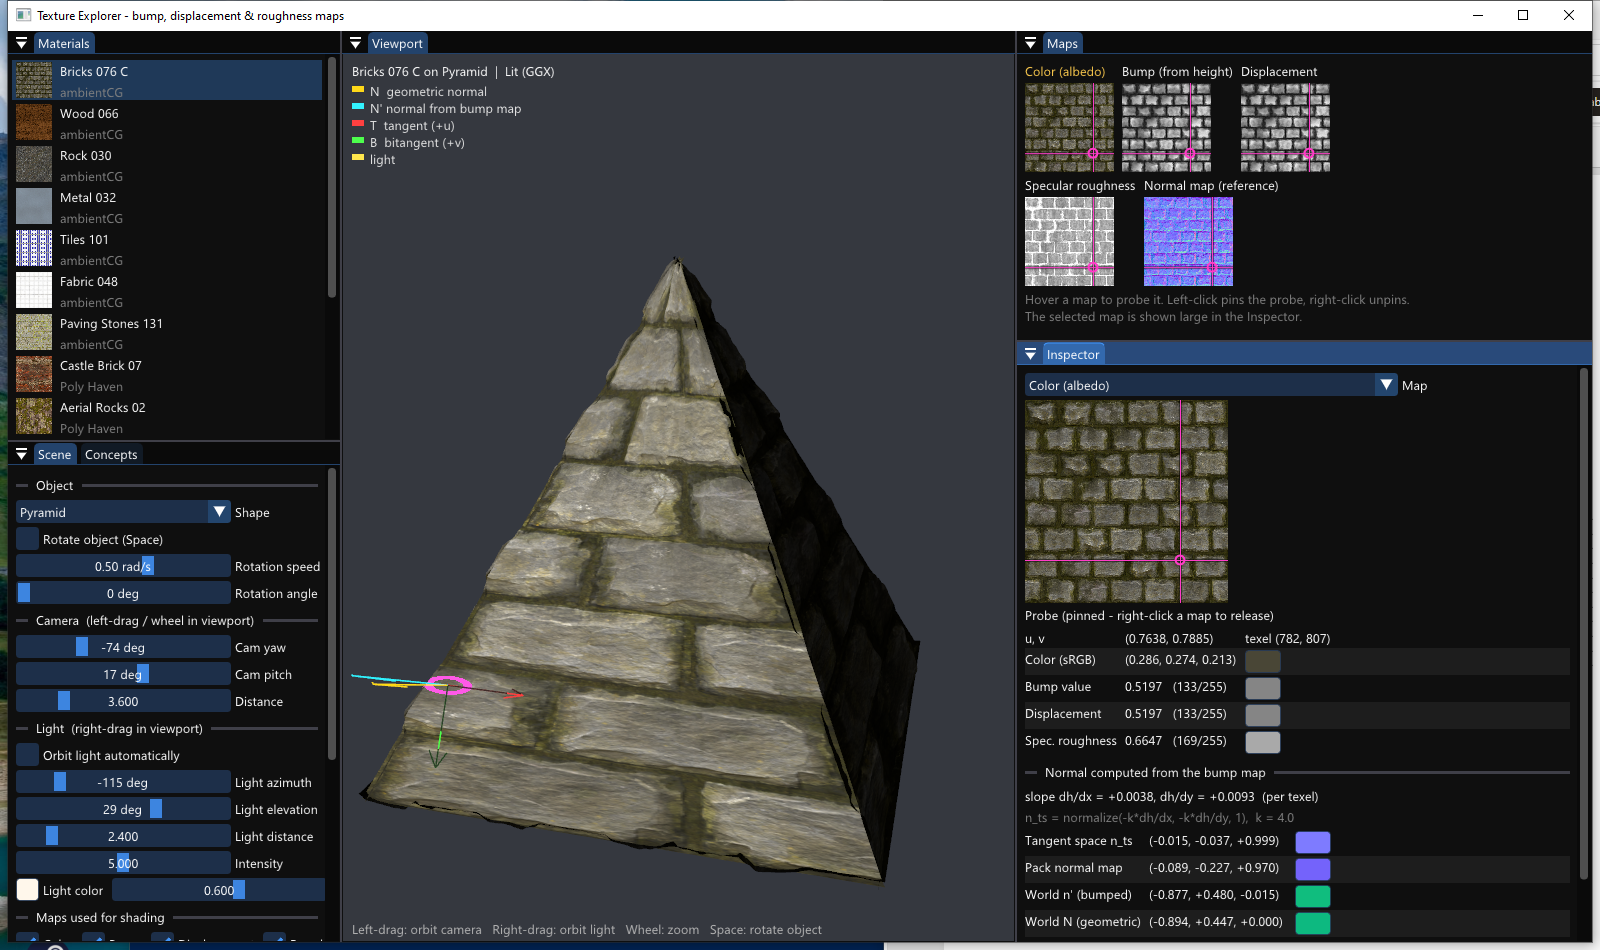
\includegraphics[width=\linewidth]{figures/pyramid-probe.png}
  \caption{Texture Explorer showing a brick material on the pyramid. The probe is pinned
  on a texel (crosshairs on every map); the Inspector lists its values and normals, and the
  3D view marks the same texel with a magenta ring and the arrows $\Nv$ (yellow),
  $\vect n'$ (cyan), $\Tv$ (red) and $\Bv$ (green).}
  \label{fig:pyramid}
\end{figure}

\section*{How this guide is organized}

Part~I develops the theory that the program illustrates. Chapter~\ref{ch:texspace}
introduces texture space and the parametrization of surfaces, using the four solids of the
program as examples. Chapter~\ref{ch:sampling} explains how a texture is sampled: texel
centres, bilinear filtering, mipmaps and colour spaces. Chapter~\ref{ch:height} is the core:
height fields used as bump maps and as displacement maps, the derivation of the perturbed
normal, and normal maps. Chapter~\ref{ch:tangent} studies the tangent frame and the
transformation of normals, and Chapter~\ref{ch:lighting} the microfacet model of reflection
through which roughness acts.

Part~II walks through the implementation. Every listing in it is extracted automatically
from the source files when this document is built, so the code shown is always the code that
runs; each listing is labelled with its file and line numbers. Chapter~\ref{ch:exercises}
proposes experiments and exercises for a course. For a broader treatment of every topic, see
the books by Akenine-M\"oller et al.\ \cite{akenine2018} and by Pharr et al.\ \cite{pharr2016}.

\section*{Running the program}

The program needs Windows 10 or later and a GPU with Direct3D~11. From the root of the
repository:

\begin{lstlisting}[language={},numbers=none,frame=none,basicstyle=\ttfamily\small]
powershell -ExecutionPolicy Bypass -File tools\fetch_textures.ps1   # once
cmake -S . -B build -G "Visual Studio 17 2022" -A x64
cmake --build build --config Release
build\Release\TextureExplorer.exe
\end{lstlisting}

The window is divided into dockable panels: \emph{Materials} (the list of materials and the
origin of the selected one), \emph{Scene} (controls), \emph{Concepts} (short explanations),
\emph{Viewport} (the 3D view), \emph{Maps} (all the maps of the material) and
\emph{Inspector} (the probe). In the viewport, dragging with the left button orbits the
camera, dragging with the right button orbits the light, the wheel zooms, and the space bar
starts or stops the rotation of the solid. On a map, hovering moves the probe, a left click
pins it, and a right click releases it.

\paragraph{Conventions.} Vectors are bold: $\vect p$, $\Nv$. Unit vectors are not marked
specially. The world is right-handed with $y$ up. Texture space follows Direct3D:
$(0,0)$ is the top-left corner of an image and $v$ grows downwards
(Section~\ref{sec:uvconv}).

\part{Theory}
\chapter{Texture space and parametric surfaces}
\label{ch:texspace}

\section{Images, texels and normalized coordinates}

A texture is an image of $W\times H$ \emph{texels}. Shaders do not address texels by
integer indices, however, but by \emph{normalized texture coordinates} $(u,v)\in[0,1]^2$,
so that the same coordinates work whatever the resolution of the image. Texel $(i,j)$, with
$0\le i<W$ and $0\le j<H$, covers the little rectangle
\[
  \Bigl[\tfrac{i}{W},\tfrac{i+1}{W}\Bigr]\times\Bigl[\tfrac{j}{H},\tfrac{j+1}{H}\Bigr],
\]
and its \emph{centre} is at $\bigl((i+\frac12)/W,\ (j+\frac12)/H\bigr)$. The distinction
between the corner and the centre of a texel matters as soon as we interpolate between texels
(Chapter~\ref{ch:sampling}); the program's probe reports both the normalized coordinates and
the integer texel $(\lfloor uW\rfloor,\lfloor vH\rfloor)$.

\begin{figure}[ht]
\centering
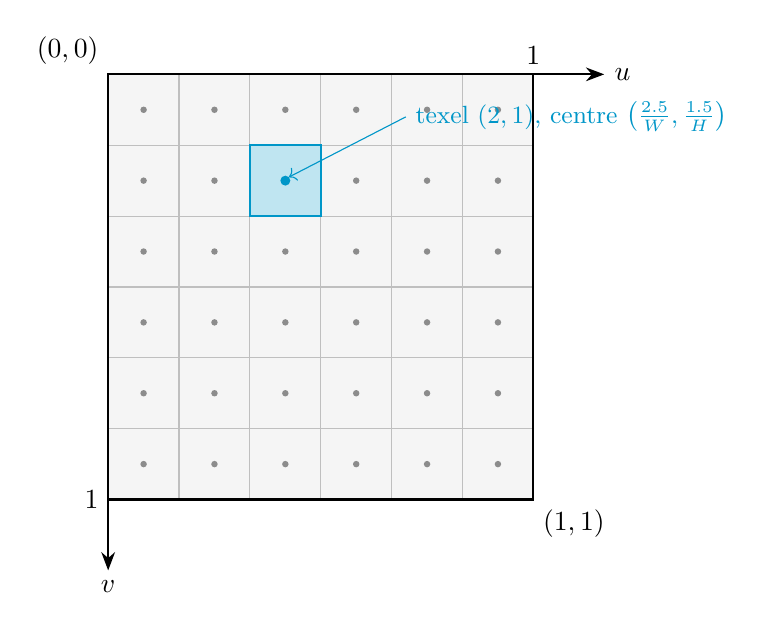
\begin{tikzpicture}[scale=0.9]
  % texel grid 6x6 in a 6x6 square
  \fill[black!4] (0,0) rectangle (6,-6);
  \draw[black!25] (0,0) grid[step=1] (6,-6);
  \draw[thick] (0,0) rectangle (6,-6);
  \foreach \i in {0,...,5} \foreach \j in {0,...,5}
    \fill[black!45] (\i+0.5,-\j-0.5) circle (1.3pt);
  % axes
  \draw[-{Stealth},thick] (0,0) -- (7,0) node[right] {$u$};
  \draw[-{Stealth},thick] (0,0) -- (0,-7) node[below] {$v$};
  \node[above left] at (0,0) {$(0,0)$};
  \node[above] at (6,0) {$1$};
  \node[left] at (0,-6) {$1$};
  \node[below right] at (6,-6) {$(1,1)$};
  % highlight texel (2,1)
  \fill[npcolor!25] (2,-1) rectangle (3,-2);
  \draw[npcolor,thick] (2,-1) rectangle (3,-2);
  \fill[npcolor] (2.5,-1.5) circle (2pt);
  \draw[npcolor,<-] (2.55,-1.45) -- (4.2,-0.6) node[right,align=left,font=\small]
     {texel $(2,1)$, centre $\bigl(\tfrac{2.5}{W},\tfrac{1.5}{H}\bigr)$};
\end{tikzpicture}
\caption{Normalized texture space in the Direct3D convention, for an image of
$W=H=6$ texels. The dots are texel centres.}
\label{fig:uvspace}
\end{figure}

\subsection{Which way is up?}
\label{sec:uvconv}
Two conventions coexist. Direct3D, Vulkan and Metal put $(0,0)$ at the \emph{top-left}
corner of the image, with $v$ growing downwards, which is the order in which image files store
their rows. OpenGL puts $(0,0)$ at the \emph{bottom-left}, with $v$ growing upwards, like a
mathematical graph. The two are related by $v_{\mathrm{GL}} = 1 - v_{\mathrm{D3D}}$.
Texture Explorer uses the Direct3D convention throughout (Figure~\ref{fig:uvspace}), which
has a pleasant side effect: the mouse position on an image on the screen, where $y$ also grows
downwards, converts to $(u,v)$ without any flip.

The convention leaves a trace in every normal map: the green channel stores the
component of the normal along $+v$, and $+v$ points down in Direct3D but up in OpenGL. That is
why material libraries ship two variants, ``NormalDX'' and ``NormalGL'', whose green channels
are inverted with respect to each other (Section~\ref{sec:normalmaps}).

\section{Parametric surfaces}

Texture mapping assigns texture coordinates to every point of a surface. For the simple
solids of Texture Explorer the natural way to do this is to describe the surface itself as a
\emph{parametric surface}, a function from a domain of the plane to space,
\[
  \vect P : [0,1]^2 \to \mathbb R^3,\qquad (u,v)\mapsto \vect P(u,v),
\]
and to use the parameters as texture coordinates. (In the program the parameters of a patch
are called $(a,b)$ and are mapped affinely to $(u,v)$; for this chapter we identify them.)

The two partial derivatives
\[
  \vect P_u = \dd{\vect P}{u},\qquad \vect P_v = \dd{\vect P}{v}
\]
are tangent to the surface: $\vect P_u$ points in the direction in which the texture's $u$
increases, and $\vect P_v$ in the direction of increasing $v$. Where they are linearly
independent, their cross product is perpendicular to the surface, and the unit normal is
\[
  \Nv = \pm\frac{\vect P_u\times\vect P_v}{\lVert\vect P_u\times\vect P_v\rVert}.
\]
The sign is chosen so that $\Nv$ points out of the solid.

\subsection{Orientation and mirrored textures}
\label{sec:orientation}
Which sign is the outward one? Imagine looking at the surface from outside. For the texture
to appear the right way round---not mirrored---$u$ must grow to the viewer's right and, with
the Direct3D convention, $v$ must grow \emph{downwards}. In a right-handed system,
right $\times$ down points \emph{into} the surface. Hence, for a correctly oriented texture,
\begin{equation}
  \label{eq:orientation}
  \vect P_u \times \vect P_v \ \text{points inwards,\quad i.e.}\quad
  \Tv\times\Bv = -\Nv
\end{equation}
where $\Tv$ and $\Bv$ are $\vect P_u$ and $\vect P_v$ normalized (and made perpendicular,
Chapter~\ref{ch:tangent}). Every shape of the program was checked against
\eqref{eq:orientation}; if it fails, the texture appears mirrored, text in it would read
backwards, and---more subtly---the normals computed from a bump map lean the wrong way.

\subsection{Distortion}
A texture is a flat image, and most surfaces cannot be flattened without stretching. How
much a parametrization stretches the texture is measured by the lengths of the derivatives and
the angle between them, collected in the \emph{first fundamental form}
\[
  E = \vect P_u\cdot\vect P_u,\qquad F = \vect P_u\cdot\vect P_v,\qquad G = \vect P_v\cdot\vect P_v .
\]
A small square $\mathrm du\times\mathrm dv$ of texture becomes, on the surface, a
parallelogram with sides $\sqrt E\,\mathrm du$ and $\sqrt G\,\mathrm dv$ and area
$\sqrt{EG-F^2}\,\mathrm du\,\mathrm dv$. The texture keeps its proportions where
$E=G$ and $F=0$ (the map is \emph{conformal} there), and keeps its scale where, in addition,
$E$ is constant.

\section{The four solids}

\begin{figure}[t]
\centering
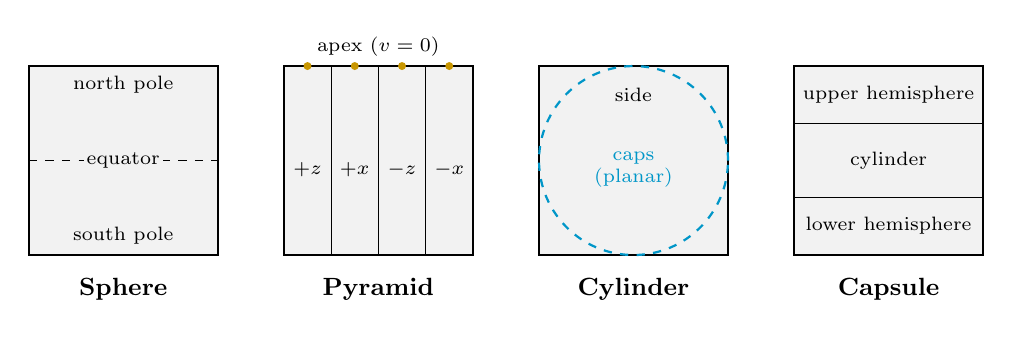
\begin{tikzpicture}[scale=2.4,font=\small]
  \tikzset{uvbox/.style={draw,thick}}
  % ---------------- sphere
  \begin{scope}[shift={(0,0)}]
    \fill[black!5] (0,0) rectangle (1,-1); \draw[uvbox] (0,0) rectangle (1,-1);
    \draw[dashed] (0,-0.5) -- (1,-0.5); \node[font=\scriptsize,fill=black!5,inner sep=1pt] at (0.5,-0.5) {equator};
    \node[font=\scriptsize] at (0.5,-0.1) {north pole};
    \node[font=\scriptsize] at (0.5,-0.9) {south pole};
    \node at (0.5,-1.18) {\textbf{Sphere}};
  \end{scope}
  % ---------------- pyramid
  \begin{scope}[shift={(1.35,0)}]
    \fill[black!5] (0,0) rectangle (1,-1); \draw[uvbox] (0,0) rectangle (1,-1);
    \foreach \k/\lab in {0/{$+z$},1/{$+x$},2/{$-z$},3/{$-x$}} {
      \draw (\k/4,0) -- (\k/4,-1);
      \node[font=\scriptsize] at (\k/4+0.125,-0.55) {\lab};
      \fill[ncolor] (\k/4+0.125,0) circle (0.6pt);
    }
    \node[font=\scriptsize,above] at (0.5,0) {apex ($v=0$)};
    \node at (0.5,-1.18) {\textbf{Pyramid}};
  \end{scope}
  % ---------------- cylinder
  \begin{scope}[shift={(2.7,0)}]
    \fill[black!5] (0,0) rectangle (1,-1); \draw[uvbox] (0,0) rectangle (1,-1);
    \draw[npcolor,dashed,thick] (0.5,-0.5) circle (0.5);
    \node[font=\scriptsize] at (0.5,-0.15) {side};
    \node[font=\scriptsize,npcolor,align=center] at (0.5,-0.55) {caps\\(planar)};
    \node at (0.5,-1.18) {\textbf{Cylinder}};
  \end{scope}
  % ---------------- capsule
  \begin{scope}[shift={(4.05,0)}]
    \fill[black!5] (0,0) rectangle (1,-1); \draw[uvbox] (0,0) rectangle (1,-1);
    \draw (0,-0.3055) -- (1,-0.3055); \draw (0,-0.6945) -- (1,-0.6945);
    \node[font=\scriptsize] at (0.5,-0.153) {upper hemisphere};
    \node[font=\scriptsize] at (0.5,-0.5) {cylinder};
    \node[font=\scriptsize] at (0.5,-0.847) {lower hemisphere};
    \node at (0.5,-1.18) {\textbf{Capsule}};
  \end{scope}
\end{tikzpicture}
\caption{How the unit square of texture space is laid out on each solid. The pyramid gives
each side face a vertical strip whose top edge collapses to the apex. The cylinder's caps
reuse the coordinates of the side through a planar projection, so they are not part of the
invertible chart. On the capsule the bands are proportional to arc length.}
\label{fig:charts}
\end{figure}

Figure~\ref{fig:charts} summarizes how each solid of the program uses texture space.
They were chosen because each one illustrates a different aspect of parametrization.

\subsection{Sphere}
With polar angle $\theta=\pi v$ (measured from the north pole) and azimuth $\varphi=2\pi u$,
\[
  \vect P(u,v) = (\sin\theta\cos\varphi,\ \cos\theta,\ -\sin\theta\sin\varphi).
\]
The minus sign in the third component makes the parametrization satisfy
\eqref{eq:orientation}. The derivatives are
\[
  \vect P_u = 2\pi\sin\theta\,(-\sin\varphi,\,0,\,-\cos\varphi),\qquad
  \vect P_v = \pi\,(\cos\theta\cos\varphi,\,-\sin\theta,\,-\cos\theta\sin\varphi),
\]
so $E = 4\pi^2\sin^2\theta$, $F=0$, $G=\pi^2$. The ratio $\sqrt E/\sqrt G = 2\sin\theta$ tells
the story of every textured globe: at the equator a square texel becomes a rectangle twice as
wide as it is tall, and towards the poles the texels are squeezed horizontally until, at the
poles themselves, a whole row of the texture collapses to a point. The program drops the scalar
factor $\sin\theta$ from $\vect P_u$ before using it as a tangent direction, so that the
direction stays defined at the poles.

\subsection{Cylinder}
The side of a cylinder of radius $r$ and height $H$,
$\vect P(u,v)=(r\cos\varphi,\ H/2-vH,\ -r\sin\varphi)$, has $E=(2\pi r)^2$, $F=0$, $G=H^2$:
constant stretch, and conformal when $2\pi r = H$. A cylinder is a \emph{developable} surface:
it can be unrolled onto the plane without distortion, which is why labels on cans look
perfect.

The caps are discs. Texture Explorer textures them with a \emph{planar projection}: the point
$(x,\pm H/2,z)$ of a cap gets the texture coordinates of its position in the square
circumscribed about the disc. The cap therefore shows a round piece of the texture, but the
same $(u,v)$ now appears on the side \emph{and} on both caps: the texture mapping is no longer
one-to-one. The probe of the program resolves this by working only with the side, the
\emph{main chart}; the shader's magenta ring around the probed texel, drawn in texture space,
appears on all three patches and makes the ambiguity visible.

\subsection{Capsule}
A capsule---a cylinder of radius $r$ and half-length $L$ capped by two hemispheres---is a
surface of revolution, described by its \emph{profile} curve in the half-plane $(\rho,y)$,
$\rho$ being the distance to the axis. The profile has three pieces: a quarter circle of length
$q=\pi r/2$, a segment of length $2L$ and another quarter circle. Texture Explorer makes $v$
proportional to the \emph{arc length} $s$ along the profile,
\[
  s = v\,(2q + 2L).
\]
With this choice $G$ is constant over the whole capsule---equal steps in $v$ are equal distances
on the surface---and the texture flows smoothly from the hemispheres onto the cylinder without
being squeezed at the junctions. With $r=L=\frac12$ the hemispheres take the bands
$v<0.3055$ and $v>0.6945$ of the texture (Figure~\ref{fig:charts}).

\subsection{Pyramid}
The pyramid shows the problem of texturing a polyhedron. One could repeat the whole texture on
each triangular face, but then every texel would appear four times on the solid and the
question ``where is this texel?'' would have four answers. Texture Explorer instead gives
each face a vertical strip of width $\frac14$ in texture space. Face $i$ goes from the apex
$\vect A$ to the base edge $c_i c_{i+1}$:
\[
  \vect P(s,t) = \vect A + t\,\bigl(\mathrm{lerp}(c_i,c_{i+1},s)-\vect A\bigr),\qquad
  u = \tfrac{i+s}{4},\quad v=t .
\]
The price is visible in the program. At the base, $\lVert\vect P_u\rVert = 4\cdot1.6 = 6.4$
while $\lVert\vect P_v\rVert\approx1.79$, so a square texel becomes a rectangle about $3.6$
times wider than tall; towards the apex the rows shrink until the strip's top edge collapses
to a point. This is a good
occasion to discuss why real models are \emph{unwrapped} into UV layouts by artists, and why
those layouts are made of many separate pieces (\emph{charts} or \emph{islands}) with seams
between them.

\subsection{Seams}
Every parametrization of a closed surface has seams. On the sphere, the cylinder and the
capsule, the line $u=0$ and the line $u=1$ are the same curve on the solid. A mesh built on a
grid of parameters therefore has two rows of vertices there, at the same positions but with
different texture coordinates, $u=0$ and $u=1$. The texture must \emph{tile} (its left and
right borders must match) for the seam to be invisible; the materials of the program are
designed to tile.

\begin{tryit}
Choose the view ``UV coordinates'' in the Scene panel. Red encodes $u$ and green encodes $v$.
On the sphere, follow the red gradient around the equator and find the seam; on the pyramid,
notice that each face has its own red gradient from $0.25k$ to $0.25(k+1)$; on the cylinder,
compare the side and the caps.
\end{tryit}

\chapter{Sampling textures}
\label{ch:sampling}

A shader asks for the value of a texture at an arbitrary point $(u,v)$, which almost never
falls on a texel centre. How the answer is computed---\emph{texture filtering}---affects both
the quality of the image and, in Texture Explorer, the agreement between the numbers the
probe computes on the CPU and the pixels the GPU draws.

\section{Addressing}
Coordinates outside $[0,1]$ are folded back according to an \emph{addressing mode}. Texture
Explorer uses \emph{wrap} (repeat): the texture tiles the plane, and texel indices are taken
modulo the size of the image. In C++, where the remainder of a negative number is negative,
the correct index is
\[
  \operatorname{wrap}(i,n) = ((i \bmod n) + n) \bmod n .
\]
Wrapping matters even inside $[0,1]$: the texels on the left border must be interpolated with
those on the right border, which is what makes tiling textures seamless.

\section{Nearest and bilinear filtering}

\begin{figure}[ht]
\centering
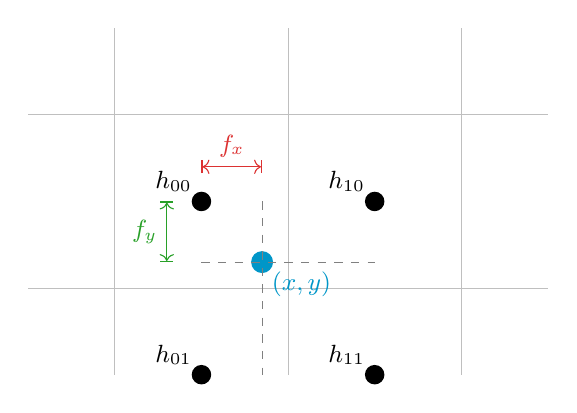
\begin{tikzpicture}[scale=2.2]
  \draw[black!25] (-0.5,0.5) grid[step=1] (2.5,-1.5);
  \foreach \x/\y/\n in {0/0/{h_{00}},1/0/{h_{10}},0/-1/{h_{01}},1/-1/{h_{11}}} {
    \fill (\x+0.5,\y-0.5) circle (1.6pt);
    \node[above left,font=\small] at (\x+0.5,\y-0.5) {$\n$};
  }
  \fill[npcolor] (0.85,-0.85) circle (1.8pt);
  \node[npcolor,below right,font=\small] at (0.85,-0.85) {$(x,y)$};
  \draw[|<->|,tcolor] (0.5,-0.3) -- node[above,font=\small] {$f_x$} (0.85,-0.3);
  \draw[|<->|,bcolor] (0.3,-0.5) -- node[left,font=\small] {$f_y$} (0.3,-0.85);
  \draw[dashed,black!50] (0.85,-0.5) -- (0.85,-1.5);
  \draw[dashed,black!50] (0.5,-0.85) -- (1.5,-0.85);
\end{tikzpicture}
\caption{Bilinear filtering interpolates the four texel centres that surround the sample
point, with weights given by the fractional offsets $f_x$, $f_y$.}
\label{fig:bilinear}
\end{figure}

\emph{Nearest} filtering returns the texel that contains the point; magnified, the texture
looks blocky. \emph{Bilinear} filtering interpolates between the four nearest texel centres.
In texel units the point is at $x = uW - \frac12$, $y = vH - \frac12$ (the $-\frac12$ moves
the origin to the first texel's centre); with $x_0=\lfloor x\rfloor$, $y_0=\lfloor y\rfloor$
and the fractions $f_x = x - x_0$, $f_y = y - y_0$,
\[
  h(x,y) = (1-f_y)\bigl[(1-f_x)\,h_{00} + f_x\,h_{10}\bigr] + f_y\bigl[(1-f_x)\,h_{01} + f_x\,h_{11}\bigr],
\]
where $h_{ab}$ is the texel $(x_0+a,\ y_0+b)$ (Figure~\ref{fig:bilinear}). Texture Explorer
implements exactly this formula on the CPU (Section~\ref{sec:cpusampling}), so that the probe
reads the same values as the GPU. The result is continuous but its derivative is not: it
jumps at texel centres, which will matter when we differentiate height maps.

\section{Minification and mipmaps}
When the texture is seen from far away, one pixel of the screen covers many texels. Sampling
just one point of that footprint is \emph{aliasing}: fine detail turns into noise that
shimmers when the camera moves. The standard remedy, \emph{mipmapping} \cite{williams1983},
precomputes a pyramid of images, each half the size of the previous one and obtained by
averaging $2\times2$ blocks, and chooses for each pixel the level whose texels are about the
size of the pixel. If $\rho$ is the number of texels of level~0 that the pixel spans, measured
with the screen-space derivatives of $(uW, vH)$,
\[
  \rho = \max\Bigl(\Bigl\lVert\dd{(uW,vH)}{x}\Bigr\rVert,\ \Bigl\lVert\dd{(uW,vH)}{y}\Bigr\rVert\Bigr),
  \qquad \lambda = \log_2 \rho ,
\]
the GPU samples level $\lambda$, interpolating between the two nearest levels
(\emph{trilinear} filtering). When the footprint is long and thin---a surface seen at a grazing
angle---a single level is either too blurry along one direction or aliased along the other;
\emph{anisotropic} filtering takes several samples along the long axis. Texture Explorer
creates every texture with its complete mipmap chain (generated by the GPU) and uses a
sampler with $8\times$ anisotropic filtering.

\paragraph{Mipmaps in a vertex shader.} The level $\lambda$ is computed from the difference
between neighbouring \emph{pixels}, which only exist in the pixel shader. A vertex shader that
reads a texture---as displacement mapping does---must choose the level itself. The right
choice depends on how densely the mesh samples the texture: Texture Explorer's meshes have
$256\times256$ cells per patch and its maps $1024\times1024$ texels, so each cell spans four
texels and the vertex shader reads level $\log_2(1024/256)=2$. Reading level~0 instead would
make the displaced surface jitter as tiny height details fall between vertices.

\paragraph{Derivatives of a texture.} The bump-mapping code of Chapter~\ref{ch:height}
samples the bump map one texel to each side of the point, always at level~0, so that the CPU
and the GPU compute the same slope. This is simple and exact but aliases when the solid is
small on the screen; a production renderer would scale the offsets with the mip level, or use
a normal map with its own mipmaps.

\section{Colour spaces}
\label{sec:srgb}

The values stored in an 8-bit colour image are not proportional to light. They are encoded with
the \emph{sRGB transfer function}, which spends more of the 256 codes on dark tones, where the
eye is more sensitive. Decoding a stored value $C\in[0,1]$ to linear light gives
\[
  C_{\mathrm{lin}} =
  \begin{cases}
    C/12.92, & C\le 0.04045,\\[2pt]
    \bigl((C+0.055)/1.055\bigr)^{2.4}, & C>0.04045,
  \end{cases}
\]
which is close to the power law $C^{2.2}$ (Figure~\ref{fig:srgb}).

\begin{figure}[ht]
\centering
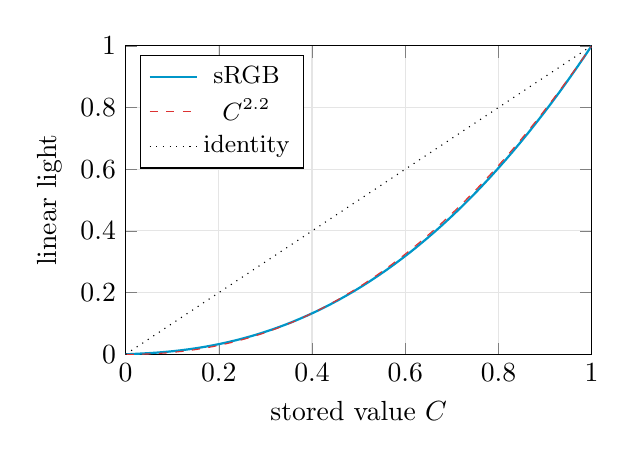
\begin{tikzpicture}
\begin{axis}[width=7.5cm,height=5.5cm,xmin=0,xmax=1,ymin=0,ymax=1,
  xlabel={stored value $C$},ylabel={linear light},legend pos=north west,
  legend style={font=\small},grid=major,grid style={black!10}]
  \addplot[domain=0:1,samples=60,thick,npcolor] {x<=0.04045 ? x/12.92 : ((x+0.055)/1.055)^2.4};
  \addlegendentry{sRGB}
  \addplot[domain=0:1,samples=60,dashed,tcolor] {x^2.2};
  \addlegendentry{$C^{2.2}$}
  \addplot[domain=0:1,samples=2,dotted,black] {x};
  \addlegendentry{identity}
\end{axis}
\end{tikzpicture}
\caption{The sRGB decoding curve and its usual approximation.}
\label{fig:srgb}
\end{figure}

Lighting computations add and multiply amounts of light, so they must work with linear values.
Hence the rules that Texture Explorer follows:
\begin{itemize}
\item The \emph{colour} map is stored in sRGB and must be decoded before lighting. The GPU does
it for free when the texture is read through a view with an \texttt{\_SRGB} format.
\item \emph{Data} maps---bump, displacement, roughness, normal---store numbers, not colours,
and must \emph{not} be decoded. They are read through a plain \texttt{UNORM} view, which
returns the stored byte divided by $255$.
\item The scene is rendered into an sRGB target: the GPU encodes the linear result when it
writes each pixel, and also when it averages the samples of multisample antialiasing, which is
therefore done correctly in linear light.
\item The user interface, which works with display values, reads both the textures and the
rendered scene through plain views, so that the stored values reach the screen untouched.
\end{itemize}
One texture, two interpretations: Direct3D allows this when the texture is created with a
\emph{typeless} format (\texttt{R8G8B8A8\_TYPELESS}) and each \emph{view} specifies how to read
it (Section~\ref{sec:typeless}).

\chapter{Height fields: displacement, bump and normal maps}
\label{ch:height}

A grey image $h(u,v)\in[0,1]$ can describe the relief of a surface: light texels are high,
dark texels are low. Such an image is a \emph{height field}, and there are two very different
ways to use it. A \emph{displacement map} moves the surface; a \emph{bump map} leaves the
surface where it is and only changes the normal used for lighting, so that the surface
\emph{looks} as if it had been moved. The materials of Texture Explorer come with a height
map labelled ``displacement'', and the program uses the same image in both roles; switching
each role on and off separately is the quickest way to understand the difference
(Figure~\ref{fig:bumpvsdisp}).

\begin{figure}[ht]
\centering
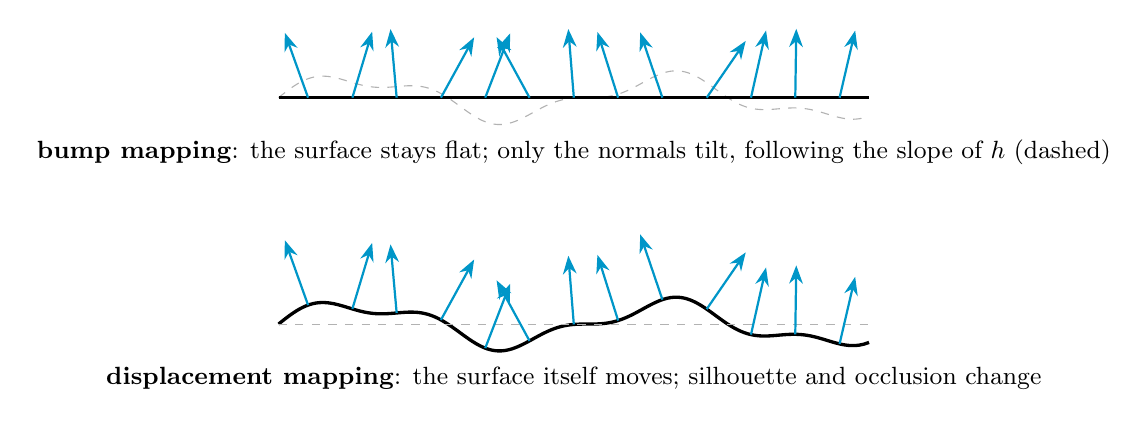
\begin{tikzpicture}[scale=1.25,
  hfun/.style={domain=0:6,samples=120,smooth}]
  % ---- bump mapping
  \begin{scope}
    \draw[black!30,dashed,hfun] plot (\x,{0.2*sin(2*\x r)+0.08*sin(5*\x r)});
    \draw[very thick] (0,0) -- (6,0);
    \foreach \x in {0.3,0.75,...,5.9} {
      \pgfmathsetmacro{\d}{0.4*cos(2*\x r)+0.4*cos(5*\x r)}
      \pgfmathsetmacro{\nx}{-\d/sqrt(1+\d*\d)}
      \pgfmathsetmacro{\ny}{1/sqrt(1+\d*\d)}
      \draw[-{Stealth},npcolor,thick] (\x,0) -- ++(0.7*\nx,0.7*\ny);
    }
    \node[font=\small] at (3,-0.55) {\textbf{bump mapping}: the surface stays flat; only the normals tilt, following the slope of $h$ (dashed)};
  \end{scope}
  % ---- displacement mapping
  \begin{scope}[shift={(0,-2.3)}]
    \draw[very thick,hfun] plot (\x,{0.2*sin(2*\x r)+0.08*sin(5*\x r)});
    \draw[black!30,dashed] (0,0) -- (6,0);
    \foreach \x in {0.3,0.75,...,5.9} {
      \pgfmathsetmacro{\h}{0.2*sin(2*\x r)+0.08*sin(5*\x r)}
      \pgfmathsetmacro{\d}{0.4*cos(2*\x r)+0.4*cos(5*\x r)}
      \pgfmathsetmacro{\nx}{-\d/sqrt(1+\d*\d)}
      \pgfmathsetmacro{\ny}{1/sqrt(1+\d*\d)}
      \draw[-{Stealth},npcolor,thick] (\x,\h) -- ++(0.7*\nx,0.7*\ny);
    }
    \node[font=\small] at (3,-0.55) {\textbf{displacement mapping}: the surface itself moves; silhouette and occlusion change};
  \end{scope}
\end{tikzpicture}
\caption{The same height field (here a sum of two sines) used in its two roles, seen in
cross-section. With bump mapping the normals are exactly those of the displaced surface,
but they are attached to the undisplaced one.}
\label{fig:bumpvsdisp}
\end{figure}

\section{Displacement mapping}
\label{sec:displacement}

Let $\vect P(u,v)$ be a surface with unit normal $\Nv(u,v)$. Displacing it by the height
field gives the new surface
\begin{equation}
  \label{eq:displace}
  \vect P'(u,v) = \vect P(u,v) + s\,\bigl(h(u,v)-m\bigr)\,\Nv(u,v),
\end{equation}
where $s$ is the \emph{displacement scale}, a length, and $m$ the \emph{mid-level}, the height
that leaves the surface in place. With the program's default $m=\frac12$, dark texels push the
surface in and light texels push it out; with $m=0$ the surface only grows.

Displacement mapping was introduced by Cook \cite{cook1984}. On the GPU it is applied per vertex in the vertex shader (Section~\ref{sec:vs}).
This is the most direct technique and has two consequences worth remembering.
\begin{itemize}
\item \emph{The mesh must be dense.} A vertex samples the height field once; detail between
vertices is lost. Texture Explorer builds every patch as a grid of $256\times256$ cells,
about $66\,000$ vertices, and samples the height at the matching mipmap level
(Chapter~\ref{ch:sampling}). Production renderers use hardware tessellation to make the mesh
dense only where it is needed.
\item \emph{Normals are not updated.} Moving the vertices does not change the normals that the
mesh carries. A displaced surface shaded with its old normals has the right silhouette and the
wrong lighting. The fix is to compute the normal of the displaced surface, which is exactly
what bump mapping does---which is why displacement and bump (or normal) maps are almost always
used together.
\end{itemize}

\paragraph{Cracks.} Equation~\eqref{eq:displace} pushes each point along \emph{its} normal.
Where a solid has a crease---the edges of the pyramid, the rims of the cylinder---the two
patches that meet there have different normals, and vertices at the same position move in
different directions: the surface tears open. Texture Explorer leaves the cracks visible on
purpose. The usual remedies are to displace along an averaged normal at the crease, or to
model creases with a small bevel.

\section{Bump mapping}
\label{sec:bump}

In 1978 James Blinn observed that the appearance of small wrinkles is due almost entirely to
the way they tilt the normal, not to the way they move the surface \cite{blinn1978}. So we can
\emph{compute} the normal of the displaced surface \eqref{eq:displace} and use it to shade the
\emph{undisplaced} one.

\subsection{Blinn's derivation}
Differentiating \eqref{eq:displace} (and writing $\tilde h = s(h-m)$),
\[
  \vect P'_u = \vect P_u + \tilde h_u\,\Nv + \tilde h\,\Nv_u,\qquad
  \vect P'_v = \vect P_v + \tilde h_v\,\Nv + \tilde h\,\Nv_v .
\]
For small bumps $\tilde h$ itself is tiny while its derivatives $\tilde h_u$, $\tilde h_v$ may
not be (a small but steep groove), so the terms $\tilde h\,\Nv_u$ and $\tilde h\,\Nv_v$ are
dropped. The normal of the displaced surface is then parallel to
\[
  \vect P'_u\times\vect P'_v \approx
  \vect P_u\times\vect P_v + \tilde h_u\,(\Nv\times\vect P_v) + \tilde h_v\,(\vect P_u\times\Nv),
\]
(the term $\tilde h_u\tilde h_v\,\Nv\times\Nv$ vanishes), which is Blinn's perturbed normal.

\subsection{In an orthonormal frame}
Suppose that, at the point, $\vect P_u = a\,\Tv$ and $\vect P_v = b\,\Bv$ with $\Tv$ and $\Bv$
orthonormal and perpendicular to $\Nv$. Then $\tilde h_u/a$ is the rate of change of the height
per unit \emph{length} along $\Tv$, and similarly $\tilde h_v/b$ along $\Bv$. Substituting
and simplifying---the result is the same whether the frame is right- or left-handed---gives
\begin{equation}
  \label{eq:bumpframe}
  \vect n' \;\propto\; \Nv \;-\; \frac{\tilde h_u}{a}\,\Tv \;-\; \frac{\tilde h_v}{b}\,\Bv .
\end{equation}
A geometric argument reaches the same result without cross products, and without worrying
about handedness. In the frame $(\Tv,\Bv,\Nv)$ the displaced surface is locally the graph
$z = g(x,y)$, whose tangent vectors are $(1,0,g_x)$ and $(0,1,g_y)$. The vector
$(-g_x,-g_y,1)$ is perpendicular to both:
\[
  (-g_x,-g_y,1)\cdot(1,0,g_x) = -g_x + g_x = 0,\qquad
  (-g_x,-g_y,1)\cdot(0,1,g_y) = -g_y + g_y = 0 .
\]
So the normal leans \emph{against} the slope: where the height increases to the right, the
normal tilts to the left. On a flat region $g_x=g_y=0$ and the normal is $(0,0,1)$, the
unperturbed $\Nv$.

\subsection{The formula used in Texture Explorer}
\label{sec:bumpformula}
Texture Explorer measures the slope in \emph{texels}: $h_x$ is the change of the bump map per
texel in the $u$ direction and $h_y$ per texel in the $v$ direction. A single \emph{bump
strength} $k$, set with a slider, converts it into a slope of the surface. The tangent-space
normal is
\begin{equation}
  \label{eq:nts}
  \nts = \frac{(-k\,h_x,\ -k\,h_y,\ 1)}{\lVert(-k\,h_x,\ -k\,h_y,\ 1)\rVert}.
\end{equation}
Comparing with \eqref{eq:bumpframe}, $k\,h_x$ plays the role of $\tilde h_u/a$, so
$k = sW/a$ where $W$ is the width of the texture in texels: $k$ hides the displacement scale
\emph{and} the stretch $a=\lVert\vect P_u\rVert$ of the parametrization. Using one $k$ for the
whole solid is a deliberate simplification: the bumps look equally deep everywhere, even where
the texture is stretched, as on the pyramid near its base. A physically exact bump map would
divide by the local stretch.

\section{Estimating the slope}
\label{sec:centraldiff}

\begin{figure}[ht]
\centering
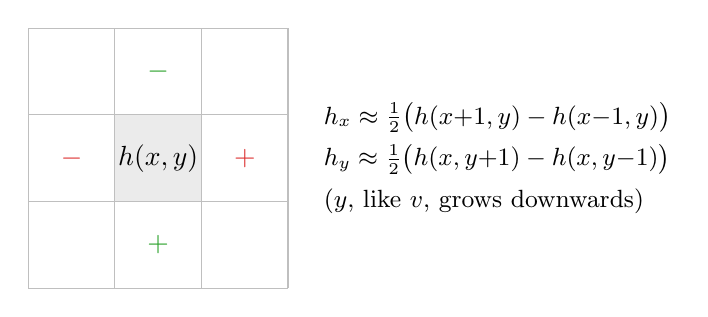
\begin{tikzpicture}[scale=1.1]
  \draw[black!25] (0,0) grid (3,3);
  \fill[black!8] (1,1) rectangle (2,2);
  \node at (1.5,1.5) {$h(x,y)$};
  \node[tcolor] at (0.5,1.5) {$-$};
  \node[tcolor] at (2.5,1.5) {$+$};
  \node[bcolor] at (1.5,2.5) {$-$};
  \node[bcolor] at (1.5,0.5) {$+$};
  \node[right,align=left,font=\small] at (3.3,1.5)
    {$h_x \approx \tfrac12\bigl(h(x{+}1,y)-h(x{-}1,y)\bigr)$\\[4pt]
     $h_y \approx \tfrac12\bigl(h(x,y{+}1)-h(x,y{-}1)\bigr)$\\[4pt]
     ($y$, like $v$, grows downwards)};
\end{tikzpicture}
\caption{The central-difference stencil. The texel itself does not take part.}
\label{fig:stencil}
\end{figure}

The derivatives of the bump map are estimated by \emph{central differences}, one texel to each
side (Figure~\ref{fig:stencil}). Taylor's theorem shows why they are preferable to the simpler
forward difference $h(x+1)-h(x)$:
\[
  \frac{h(x+1)-h(x-1)}{2} = h'(x) + \frac{h'''(x)}{6} + \dots,\qquad
  h(x+1)-h(x) = h'(x) + \frac{h''(x)}{2} + \dots
\]
The central difference is exact for quadratics and does not shift the normal by half a texel.
Both the shader and the CPU probe take the four samples with bilinear filtering at offsets of
exactly one texel, so they agree to rounding error.

\begin{tryit}
Pin the probe on the edge of a brick. Read the slopes $h_x$, $h_y$ and the tangent-space
normal in the Inspector and check equation \eqref{eq:nts} by hand: with $k=4$,
$h_x=0.0038$ and $h_y=0.0093$ give $\nts\approx(-0.015,-0.037,0.999)$. Then change the bump
strength and watch the cyan arrow $\vect n'$ in the 3D view lean further.
\end{tryit}

\section{Normal maps}
\label{sec:normalmaps}

Computing derivatives in the shader costs four texture reads per pixel. A \emph{normal map}
stores the result instead: each texel holds $\nts$, encoded as a colour by
\[
  \mathit{rgb} = \tfrac12\,\nts + \tfrac12,\qquad \nts = 2\,\mathit{rgb}-1 .
\]
Because the normals of a mostly flat surface are close to $(0,0,1)$, normal maps have the
characteristic lavender colour $(0.5,0.5,1)$. They are usually not computed from a height map
but \emph{baked} from a detailed (``high-poly'') model onto a simple one, and can represent
details that are not height fields at all, such as overhangs.

Two conventions exist, differing in the sign of the green channel (Section~\ref{sec:uvconv}):
\emph{DirectX} normal maps store the component along $+v$ with $v$ downwards, \emph{OpenGL}
ones along $+v$ with $v$ upwards. Using a map of the wrong convention makes the relief look
lit from below. Texture Explorer's tangent-space $y$ axis is $+v$ downwards, so it decodes the
DirectX variant directly; the Inspector shows it next to the normal computed from the bump
map. The numbers differ---the authors of the material baked their map with their own strength
and from their own high-resolution geometry---but the direction in which the normal leans
agrees, which is a good check of the conventions.

Normal maps have a subtle filtering problem: averaging unit vectors (as mipmapping does)
produces shorter vectors, and renormalizing them loses the information that the surface was
bumpy at that scale. Advanced techniques (Toksvig's, or LEAN mapping) turn that lost length into
extra roughness.

\section{Summary}

\begin{table}[ht]
\centering\small
\begin{tabularx}{\linewidth}{@{}l>{\raggedright}X>{\raggedright}X>{\raggedright\arraybackslash}X@{}}
\toprule
 & \textbf{Bump map} & \textbf{Normal map} & \textbf{Displacement map}\\
\midrule
Stores & height $h$ & tangent-space normal $\nts$ & height $h$\\
Changes the shading normal & yes, from the slope of $h$ & yes, directly & no (unless normals are recomputed)\\
Changes silhouette and occlusion & no & no & yes\\
Cost & 4 extra samples per pixel & 1 sample per pixel & dense mesh or tessellation\\
Typical artefacts & flat silhouettes; light leaking on the dark side & same, plus wrong green convention & cracks at creases; swimming if under-sampled\\
In Texture Explorer & \code{BumpNormalTS} in the pixel shader & shown for comparison only & \code{VSMain} in the vertex shader\\
\bottomrule
\end{tabularx}
\caption{Three ways to use relief in a material.}
\label{tab:reliefs}
\end{table}

Bump and normal maps share one more artefact. A perturbed normal may face the light at points
where the real surface faces away from it, so the dark side of the solid sparkles. Texture
Explorer attenuates the lighting with a steep ramp of the \emph{geometric} cosine
$\Nv\cdot\vect L$ (Section~\ref{sec:horizon}), a crude form of self-shadowing.

\chapter{Tangent space}
\label{ch:tangent}

Equation~\eqref{eq:nts} gives the bumped normal in coordinates relative to the surface. To
light the surface we need it in the same coordinate system as the light and the camera. This
chapter is about the frame that connects the two, and about transforming normals in general.

\section{The tangent frame}

\begin{figure}[ht]
\centering
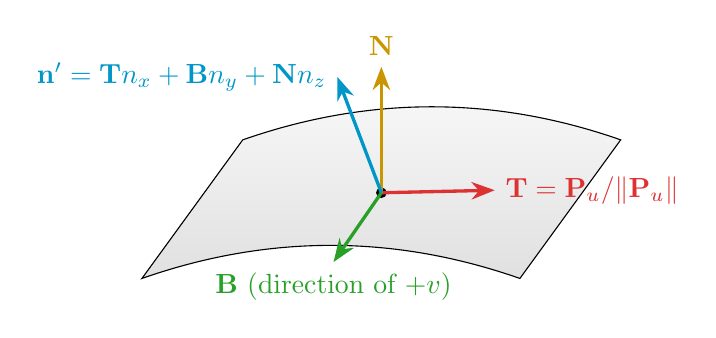
\begin{tikzpicture}[scale=1.6,>={Stealth}]
  % a curved patch drawn in a simple oblique projection
  \shade[top color=black!3,bottom color=black!12]
    (0,0) .. controls (1,0.35) and (2,0.35) .. (3,0)
    -- (3.8,1.1) .. controls (2.8,1.45) and (1.8,1.45) .. (0.8,1.1) -- cycle;
  \draw (0,0) .. controls (1,0.35) and (2,0.35) .. (3,0)
    -- (3.8,1.1) .. controls (2.8,1.45) and (1.8,1.45) .. (0.8,1.1) -- cycle;
  \coordinate (p) at (1.9,0.68);
  \fill (p) circle (1.2pt);
  \draw[->,very thick,tcolor] (p) -- ++(0.9,0.02) node[right] {$\Tv=\vect P_u/\lVert\vect P_u\rVert$};
  \draw[->,very thick,bcolor] (p) -- ++(-0.38,-0.55) node[below] {$\Bv$ (direction of $+v$)};
  \draw[->,very thick,ncolor] (p) -- ++(0,1.0) node[above] {$\Nv$};
  \draw[->,very thick,npcolor] (p) -- ++(-0.35,0.92) node[left] {$\vect n' = \Tv n_x+\Bv n_y+\Nv n_z$};
\end{tikzpicture}
\caption{The tangent frame at a point of a surface: $\Tv$ along increasing $u$, $\Bv$
along increasing $v$, $\Nv$ outwards. A tangent-space vector $(n_x,n_y,n_z)$ is the
combination $n_x\Tv+n_y\Bv+n_z\Nv$.}
\label{fig:tbn}
\end{figure}

At each point of a textured surface we attach three unit vectors (Figure~\ref{fig:tbn}):
the \emph{tangent} $\Tv$, in the direction of increasing $u$; the \emph{bitangent} $\Bv$
(sometimes, inaccurately, called the binormal), in the direction of increasing $v$; and the
normal $\Nv$. A vector with tangent-space coordinates $\nts=(n_x,n_y,n_z)$ is, in object
coordinates,
\[
  \vect n_{\mathrm{obj}} = n_x\,\Tv + n_y\,\Bv + n_z\,\Nv =
  \underbrace{\begin{pmatrix}\Tv & \Bv & \Nv\end{pmatrix}}_{\text{TBN}}
  \begin{pmatrix}n_x\\ n_y\\ n_z\end{pmatrix}.
\]
This is the famous \emph{TBN matrix}. When its columns are orthonormal, its inverse is its
transpose, so going back---from object space to tangent space, as some techniques do with the
light vector---costs three dot products.

The tangent frame is the reason a single bump or normal map works on any shape: the map
describes the relief \emph{relative to the surface}, and the frame carries it onto whatever
surface it is applied to.

\section{Building an orthonormal frame}

The derivatives $\vect P_u$ and $\vect P_v$ of a parametrization are tangent to the surface but
in general neither unit nor perpendicular (think of the pyramid, Chapter~\ref{ch:texspace}).
Texture Explorer builds an orthonormal frame by the \emph{Gram--Schmidt} process:
\begin{align*}
  \Nv &= \text{the unit outward normal},\\
  \Tv &= \frac{\vect P_u - (\vect P_u\cdot\Nv)\,\Nv}{\lVert\vect P_u - (\vect P_u\cdot\Nv)\,\Nv\rVert},\\
  \Bv &= \sigma\,(\Nv\times\Tv),\qquad \sigma = \operatorname{sign}\bigl((\Nv\times\Tv)\cdot\vect P_v\bigr).
\end{align*}
The sign $\sigma$---stored as the fourth component $w$ of the vertex tangent---records the
\emph{handedness} of the frame. It is needed because a texture can be applied mirrored; with
the conventions of this program, \eqref{eq:orientation} gives $\Tv\times\Bv=-\Nv$ and so
$\sigma=-1$ everywhere. Storing $\Tv$ and $\sigma$ instead of $\Tv$ and $\Bv$ saves two floats
per vertex.

\paragraph{After interpolation.} The rasterizer interpolates $\Nv$ and $\Tv$ linearly across
each triangle. Interpolated unit vectors are shorter than one and no longer perpendicular, so the
pixel shader repeats the Gram--Schmidt step before using them. In production, normal maps are
baked against a precisely specified tangent frame---the \emph{MikkTSpace} convention
\cite{mikkelsen2008}---and the renderer must reproduce exactly the same frame, or the baked
normals come out slightly wrong.

\section{A worked example}
Take the sphere of Chapter~\ref{ch:texspace} at the centre of the texture, $u=v=\frac12$, so
$\theta=\pi/2$ and $\varphi=\pi$. Then
\begin{align*}
  \vect P &= (-1,0,0) = \Nv,\\
  \Tv &= (-\sin\varphi,\,0,\,-\cos\varphi) = (0,0,1),\\
  \Bv &= (\cos\theta\cos\varphi,\,-\sin\theta,\,-\cos\theta\sin\varphi) = (0,-1,0).
\end{align*}
Check the orientation: $\Tv\times\Bv = (0,0,1)\times(0,-1,0) = (1,0,0) = -\Nv$. A tangent-space
normal $\nts = (0.1,\,0,\,0.995)$, leaning towards $+u$, becomes
\[
  \vect n' = 0.1\,\Tv + 0.995\,\Nv = (-0.995,\ 0,\ 0.1)
\]
in object space: it leans towards $+z$, the direction in which $u$ grows at that point. This is
exactly what the Inspector shows when the probe is placed there (with the solid not rotated).

\section{Transforming normals}
\label{sec:normaltransform}

Points and tangent vectors of an object are transformed to the world by its world matrix $M$
(more precisely, by its upper-left $3\times3$ part for vectors). Normals are different. A normal
is defined by being perpendicular to all tangent vectors $\vect t$: $\vect n\cdot\vect t = 0$.
If tangents are transformed as $\vect t' = M\vect t$, the transformed normal must satisfy
$\vect n'\cdot M\vect t = 0$ for every $\vect t$, which holds for
\[
  \vect n' = M^{-\mathsf T}\vect n,\qquad\text{since}\qquad
  (M^{-\mathsf T}\vect n)\cdot(M\vect t) = \vect n^{\mathsf T}M^{-1}M\vect t = \vect n\cdot\vect t = 0 .
\]
For a non-uniform scale, $M^{-\mathsf T}\neq M$ and using $M$ for normals is a classic bug: the
normals of a squashed sphere would lean the wrong way. For a \emph{rotation},
$M^{-\mathsf T}=M$, and for a uniform scale they differ only by a factor that normalization
removes. Texture Explorer's world matrix is a pure rotation about the vertical axis (the
rotation animation), so it transforms points, tangents and normals with the same matrix.

\begin{tryit}
Pin the probe, then start the rotation of the object (space bar). The world-space vectors in
the Inspector change continuously, while the tangent-space normal stays the same: the relief is
a property of the surface, the world-space normal a property of the surface \emph{and} its
placement in the world.
\end{tryit}

\chapter{Lighting and specular roughness}
\label{ch:lighting}

The bumped normal and the roughness map only become visible through the lighting model. Texture
Explorer uses the microfacet model that real-time graphics has adopted as its standard
\cite{cook1982,walter2007,karis2013}. This chapter states it, explains each factor, and shows
where roughness enters.

\section{Reflection from a point light}
The program lights the solid with a single point light at position $\vect p_L$ with colour and
intensity $E$. At a surface point $\vect x$ with (bumped) normal $\vect n$, let
\[
  \vect L = \frac{\vect p_L-\vect x}{\lVert\vect p_L-\vect x\rVert},\qquad
  \vect V = \frac{\vect p_{\mathrm{eye}}-\vect x}{\lVert\vect p_{\mathrm{eye}}-\vect x\rVert}
\]
be the directions to the light and to the eye. The reflected radiance is
\[
  L_o = f(\vect L,\vect V)\;E\;(\vect n\cdot\vect L)^+ \;+\; L_{\mathrm{ambient}},
\]
where $f$ is the \emph{bidirectional reflectance distribution function} (BRDF) and $(\cdot)^+$
clamps negative values to zero. (A physical point light would also fall off as the inverse
square of the distance; the program omits it so that orbiting the light does not change the
brightness.) Every $\vect n$ in this chapter is the normal from the bump map: that is how bump
mapping changes the image.

\section{Diffuse reflection}
Light that enters the material, scatters inside and comes out again leaves in all directions
equally. That is Lambert's law, with BRDF
\[
  f_d = \frac{\rho}{\pi},
\]
where $\rho$ is the \emph{albedo}, read from the colour map and decoded from sRGB. The
$1/\pi$ makes the surface reflect at most all the light it receives.

\section{Specular reflection: microfacets}

\begin{figure}[ht]
\centering
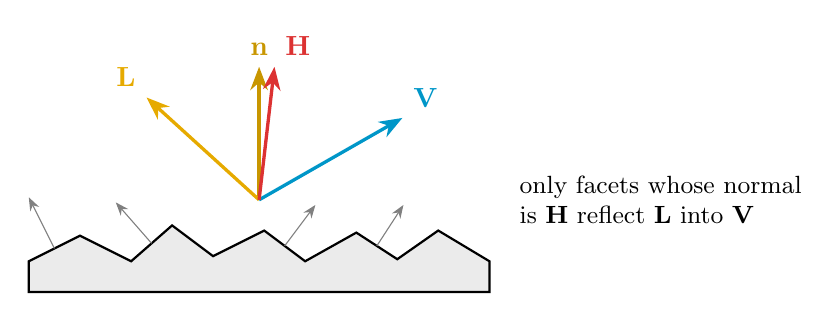
\begin{tikzpicture}[scale=1.3,>={Stealth}]
  \draw[thick,fill=black!8] (0,0) -- (0.5,0.25) -- (1,0) -- (1.4,0.35) -- (1.8,0.05) -- (2.3,0.3)
     -- (2.7,0) -- (3.2,0.28) -- (3.6,0.02) -- (4,0.3) -- (4.5,0) -- (4.5,-0.3) -- (0,-0.3) -- cycle;
  % facet normals
  \foreach \a/\b/\c/\d in {0/0/0.5/0.25, 1/0/1.4/0.35, 2.3/0.3/2.7/0, 3.2/0.28/3.6/0.02} {
    \draw[->,black!50] ($(\a,\b)!0.5!(\c,\d)$) -- ++($ (\b,-\a) - (\d,-\c) $);
  }
  % macro normal, L, V, H at a facet whose normal is along H
  \coordinate (x) at (1.2,0.175);
  \draw[->,very thick,ncolor] (2.25,0.6) -- ++(0,1.3) node[above] {$\vect n$};
  \draw[->,very thick,lcolor] (2.25,0.6) -- ++(-1.1,1.0) node[above left] {$\vect L$};
  \draw[->,very thick,npcolor] (2.25,0.6) -- ++(1.4,0.8) node[above right] {$\vect V$};
  \draw[->,very thick,tcolor] (2.25,0.6) -- ++(0.15,1.3) node[above right] {$\vect H$};
  \node[font=\small,align=left,right] at (4.7,0.6) {only facets whose normal\\ is $\vect H$
    reflect $\vect L$ into $\vect V$};
\end{tikzpicture}
\caption{The microfacet view of a rough surface: many tiny mirrors (grey normals). The half
vector $\vect H$ is the facet orientation that reflects light from $\vect L$ towards $\vect V$.}
\label{fig:microfacets}
\end{figure}

A glossy surface is modelled as a multitude of microscopic mirrors, the \emph{microfacets},
whose orientations vary around the normal $\vect n$ (Figure~\ref{fig:microfacets}). A mirror
reflects light from $\vect L$ into $\vect V$ only if its normal is the \emph{half vector}
\[
  \vect H = \frac{\vect L+\vect V}{\lVert\vect L+\vect V\rVert}.
\]
The Cook--Torrance specular BRDF \cite{cook1982} counts those mirrors:
\[
  f_s(\vect L,\vect V) = \frac{D(\vect H)\;G(\vect L,\vect V)\;F(\vect V,\vect H)}
                              {4\,(\vect n\cdot\vect L)\,(\vect n\cdot\vect V)} .
\]
\begin{itemize}
\item $D$, the \emph{normal distribution function}, is the density of microfacets oriented
along $\vect H$. It is where \textbf{roughness} enters.
\item $G$, the \emph{geometric} or \emph{masking--shadowing} term, is the fraction of those
microfacets that are visible both from the light and from the eye.
\item $F$, the \emph{Fresnel} term, is the fraction of light that a mirror reflects, which grows
towards grazing angles.
\end{itemize}

\subsection{The GGX distribution}
Texture Explorer uses the GGX (Trowbridge--Reitz) distribution \cite{walter2007},
\[
  D(\vect H) = \frac{\alpha^2}{\pi\,\bigl((\vect n\cdot\vect H)^2(\alpha^2-1)+1\bigr)^2},
  \qquad \alpha = r^2,
\]
where $r\in[0,1]$ is the value of the roughness map. For small $\alpha$ the distribution is a
tall, narrow peak around $\vect n$: nearly all facets face the same way and the highlight is
small and bright. As $\alpha$ grows the peak spreads and lowers; at $\alpha=1$, $D=1/\pi$ is
constant and there is no highlight at all, only a sheen (Figure~\ref{fig:ggx}). GGX has longer
``tails'' than older models such as Blinn--Phong, which gives highlights the soft halo seen on
real materials. The remapping $\alpha=r^2$, popularized by Disney and Epic Games
\cite{karis2013}, makes equal steps of $r$ look like equal steps of glossiness, which is better
both for artists painting roughness maps and for a slider.

\begin{figure}[ht]
\centering
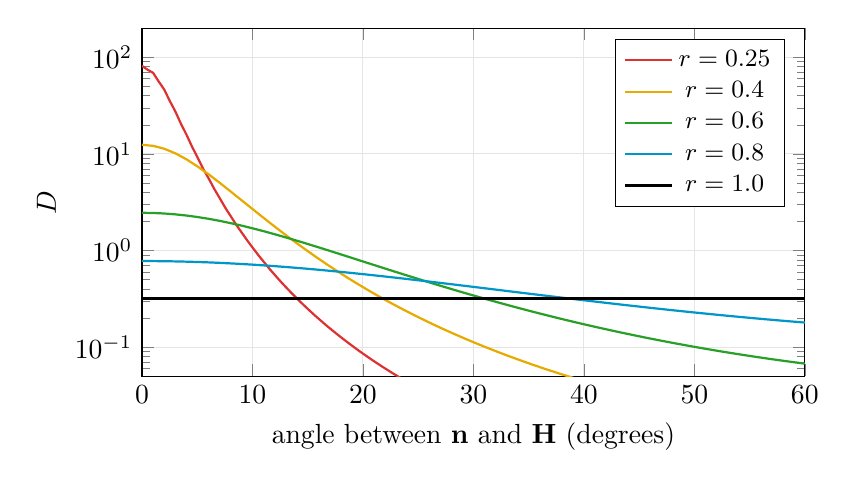
\begin{tikzpicture}
\begin{semilogyaxis}[width=10cm,height=6cm,xmin=0,xmax=60,ymin=0.05,ymax=200,
  xlabel={angle between $\vect n$ and $\vect H$ (degrees)},ylabel={$D$},
  legend style={font=\small},legend pos=north east,grid=major,grid style={black!10}]
  \foreach \r/\c in {0.25/tcolor,0.4/lcolor,0.6/bcolor,0.8/npcolor,1.0/black} {
    \edef\temp{\noexpand\addplot[thick,\c,domain=0:60,samples=120]
      {(\r^4)/(pi*((cos(x)^2)*(\r^4-1)+1)^2)};
      \noexpand\addlegendentry{$r=\r$}}
    \temp
  }
\end{semilogyaxis}
\end{tikzpicture}
\caption{The GGX distribution $D$ as a function of the angle between the normal and the half
vector, for several values $r$ of the roughness map ($\alpha=r^2$). Note the logarithmic
scale: the peak value $1/(\pi\alpha^2)$ is about $81$ at $r=0.25$ but only $2.5$ at $r=0.6$.}
\label{fig:ggx}
\end{figure}

\subsection{Masking and shadowing}
On a rough surface some facets hide others. The program uses Schlick's approximation of Smith's
masking function, with the constant $k=(r+1)^2/8$ recommended for analytic lights
\cite{karis2013}; Heitz \cite{heitz2014} explains the theory behind these functions:
\[
  G = G_1(\vect n\cdot\vect V)\,G_1(\vect n\cdot\vect L),\qquad
  G_1(c) = \frac{c}{c\,(1-k)+k}.
\]

\subsection{Fresnel reflectance}
Schlick's approximation \cite{schlick1994} interpolates between the reflectance at normal
incidence, $F_0$, and total reflection at grazing incidence:
\[
  F = F_0 + (1-F_0)\,(1-\vect V\cdot\vect H)^5 .
\]
For dielectrics (stone, wood, plastic) $F_0\approx0.04$ and is colourless; for metals $F_0$ is
high and coloured. The \emph{metallic workflow} interpolates between the two with a
\emph{metallic} parameter $\mu$: $F_0 = \mathrm{lerp}(0.04, \rho, \mu)$, and metals have no
diffuse reflection.

\section{The complete model}
Putting the pieces together, the pixel shader computes
\[
  L_o = \Bigl[(1-F)(1-\mu)\,\frac{\rho}{\pi} + \frac{D\,G\,F}{4\,(\vect n\cdot\vect L)(\vect n\cdot\vect V)}\Bigr]
        \,E\,(\vect n\cdot\vect L)^+\;\eta \;+\; a\,\rho,
\]
where the factor $1-F$ removes from the diffuse part the light already reflected specularly,
$a$ is a small ambient term, and $\eta$ is the horizon factor of the next section.

\subsection{The horizon factor}
\label{sec:horizon}
The bumped normal $\vect n$ can face the light even where the \emph{geometric} normal $\Nv$ faces
away from it; the result is light on the dark side of the solid, which looks wrong. Texture
Explorer multiplies by
\[
  \eta = \operatorname{saturate}\bigl(8\,(\Nv\cdot\vect L)\bigr),
\]
which fades the lighting out over the last few degrees before the geometric terminator. It is
a cheap stand-in for the self-shadowing of the relief.

\begin{tryit}
Choose a material whose roughness tile shows strong contrast (dark texels are glossy,
light ones rough). Orbit the light (right-drag) and watch the highlight break up: it stays on
the dark regions of the roughness map and vanishes on the light ones; the probe tells you the
roughness value under any point. Then untick ``Roughness'' and move the ``Constant roughness'' slider to
see the whole surface go from mirror-like to matte.
\end{tryit}

\part{Implementation}
\chapter{Architecture of the program}
\label{ch:architecture}

Texture Explorer is about 1\,800 lines of C++20 and HLSL. It uses three small libraries:
Dear ImGui for the user interface, \code{stb\_image} to decode images, and \code{nlohmann/json}
to read the list of materials. All three are fetched by CMake when the project is configured.

\section{Modules}

\begin{table}[ht]
\centering\small
\begin{tabularx}{\linewidth}{@{}l>{\raggedright\arraybackslash}X@{}}
\toprule
\textbf{Files} & \textbf{Responsibility}\\
\midrule
\file{src/Mesh.h}, \file{.cpp} & Parametric patches of the four solids; mesh generation; tangent frames; inverting the texture mapping\\
\file{src/Material.h}, \file{.cpp} & The manifest of materials; loading images into GPU textures and CPU copies; bilinear sampling on the CPU\\
\file{src/Inspector.h}, \file{.cpp} & The probe: map values, slope, tangent-space and world-space normals at a texel\\
\file{shaders/pbr.hlsl} & Displacement (vertex shader); bump mapping and GGX lighting (pixel shader); debug views\\
\file{shaders/gizmo.hlsl} & Coloured lines for the arrows of the probe and the light marker\\
\file{src/Renderer.h}, \file{.cpp} & Direct3D~11 device, swap chain, shader compilation, off-screen multisampled target, draw calls\\
\file{src/App.h}, \file{.cpp} & Application state and the six panels of the user interface\\
\file{src/main.cpp} & Window, Dear ImGui set-up, main loop\\
\file{tools/fetch\_textures.ps1} & Downloads the ten materials and writes \file{assets/materials/manifest.json}\\
\bottomrule
\end{tabularx}
\caption{The source files of Texture Explorer.}
\label{tab:modules}
\end{table}

\section{One frame}

\begin{figure}[ht]
\centering
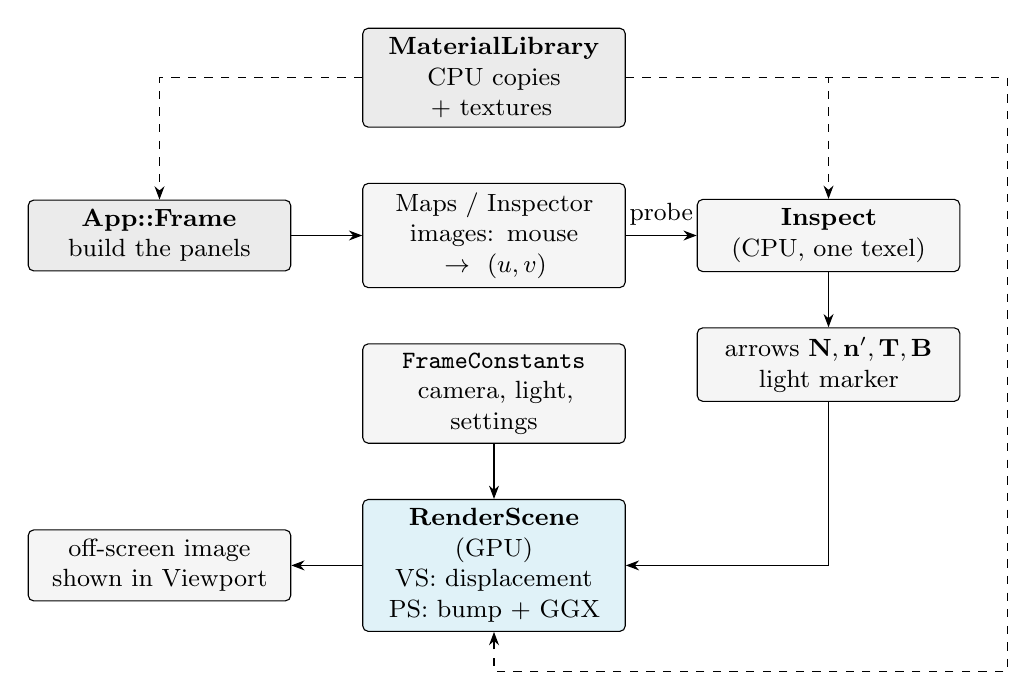
\begin{tikzpicture}[node distance=7mm and 9mm,font=\small,
  box/.style={draw,rounded corners=2pt,fill=#1,align=center,minimum height=9mm,text width=31mm},
  box/.default=black!4, >={Stealth}]
  \node[box=black!8] (ui) {\textbf{App::Frame}\\build the panels};
  \node[box,right=of ui] (maps) {Maps / Inspector\\images: mouse $\to(u,v)$};
  \node[box,right=of maps] (insp) {\textbf{Inspect}\\(CPU, one texel)};
  \node[box,below=of insp] (lines) {arrows $\Nv,\vect n',\Tv,\Bv$\\light marker};
  \node[box,below=of maps] (fc) {\code{FrameConstants}\\camera, light, settings};
  \node[box=npcolor!12,below=of fc] (gpu) {\textbf{RenderScene} (GPU)\\VS: displacement\\PS: bump + GGX};
  \node[box,left=of gpu] (img) {off-screen image\\shown in Viewport};
  \node[box=black!8,above=of maps] (lib) {\textbf{MaterialLibrary}\\CPU copies + textures};
  \draw[->] (ui) -- (maps);
  \draw[->] (maps) -- node[above]{probe} (insp);
  \draw[->] (insp) -- (lines);
  \draw[->] (lines) |- (gpu);
  \draw[->] (fc) -- (gpu);
  \draw[->] (gpu) -- (img);
  \draw[->,dashed] (lib) -| (ui);
  \draw[->,dashed] (lib) -| (insp);
  \draw[->,dashed] (lib.east) -- (lib.east -| insp.east) -- ++(0.6,0)
     |- ($(gpu.south)+(0,-0.5)$) -- (gpu.south);
\end{tikzpicture}
\caption{The flow of one frame. The same material data feeds the probe (on the CPU) and the
renderer (on the GPU), which apply the same formulas.}
\label{fig:frame}
\end{figure}

Dear ImGui is an \emph{immediate-mode} library: the user interface is not a tree of widget
objects but a function that runs every frame and calls \code{ImGui::Button},
\code{ImGui::SliderFloat}, and so on. Each call draws a widget and tells whether the user
interacted with it. The application's state therefore lives in ordinary member variables that
the rest of the program reads directly. One frame proceeds as follows
(Figure~\ref{fig:frame}):
\begin{enumerate}
\item The animations advance by the elapsed time.
\item The panels are built. While the \emph{Maps} and \emph{Inspector} panels draw their images,
they convert the mouse position into texture coordinates and update the \emph{probe}.
\item If the probe is valid, \code{Inspect} computes everything about that texel, on the CPU.
\item The \emph{Viewport} panel fills a constant buffer with the camera, the light and the
settings, adds the inspector's arrows to a list of lines, and asks the renderer to draw the scene
into an off-screen image of the size of the panel. It then shows that image.
\item Dear ImGui draws the whole interface into the window, and the frame is presented.
\end{enumerate}

\section{A design principle: compute it twice}
The pixel shader computes the bumped normal for millions of pixels and shows only the result.
To make the computation visible, the probe repeats it on the CPU for one texel and shows every
intermediate value. The two implementations must agree exactly, so they are written to be
identical:
\begin{itemize}
\item the CPU keeps a byte-for-byte copy of every map and samples it bilinearly with the GPU's
texel-centre convention (Section~\ref{sec:cpusampling});
\item the slope is estimated with the same central differences, at level~0, with the same
strength (\code{BumpNormalTangent} in C++, \code{BumpNormalTS} in HLSL);
\item the tangent frame is built with the same Gram--Schmidt construction from the same patch
functions (\code{TangentFrame} and the pixel shader);
\item the 3D position of the probe comes from the same parametric functions that generated the
mesh, so the arrows land on the pixels that show the probed texel.
\end{itemize}
The probe and the image disagree only where the program simplifies on purpose. For example, the
probe evaluates the exact surface, while the GPU draws a mesh of flat triangles.

\chapter{Geometry: patches, meshes and tangent frames}
\label{ch:geometry}

This chapter implements Chapter~\ref{ch:texspace}. The key abstraction is the \emph{patch}: a
function from the parameter square to a surface point with everything the rest of the program
needs to know about it.

\section{Surface points, vertices and patches}

A patch returns a \code{SurfacePoint}: position, unit normal, the derivatives
$\vect P_u$ and $\vect P_v$ (not normalized), and the texture coordinates. The GPU receives a
more compact \code{Vertex}, which stores the tangent made perpendicular to the normal, and the
handedness sign $\sigma$ of Chapter~\ref{ch:tangent} in its fourth component:

\excerpt{vertex}

A \code{Patch} wraps the function. When the patch's texture coordinates are an affine function of
its parameters, $u = u_0 + a(u_1-u_0)$, $v=v_0+b(v_1-v_0)$, the patch is \emph{invertible}: from
$(u,v)$ we can recover $(a,b)$ and so the point. The caps of the cylinder and the base of the
pyramid, textured by projection, are not invertible.

\excerpt{patch}

\section{The four solids}

The sphere is a direct transcription of the formulas of Chapter~\ref{ch:texspace}. Note that the
tangent passed to \code{Make} is $\vect P_u/(2\pi\sin\theta)$, which remains defined at the
poles:

\excerpt{sphere}

The cylinder has three patches. The caps compute their texture coordinates from their positions
(the planar projection); the sign \code{ny} handles the top cap (seen from above) and the bottom
cap (seen from below) with one function, keeping $\Tv\times\Bv=-\Nv$ on both:

\excerpt{cylinder}

The capsule is a surface of revolution with $v$ proportional to arc length along the profile.
For each of the three pieces of the profile the code computes the profile point
$(\rho,y)$ (\code{radial}, \code{y}), the profile normal (\code{nr}, \code{ny}), and the
profile's unit tangent $(\mathrm d\rho/\mathrm ds,\ \mathrm dy/\mathrm ds)$ (\code{dr},
\code{dy}). The revolution by the azimuth then yields the point, the normal and $\vect P_v$:

\excerpt{capsule}

Each side face of the pyramid is the family of segments from the apex to the points of the base
edge. The face normal is computed once, as $\vect B\times\vect T$ (our orientation rule read
backwards), from the edge and the median of the face:

\excerpt{pyramid}

\section{The tangent frame}
\code{TangentFrame} implements the Gram--Schmidt construction of Chapter~\ref{ch:tangent}. If
$\vect P_u$ is degenerate (zero, or parallel to $\Nv$) it derives a tangent from $\vect P_v$
instead. The bitangent is $\pm\Nv\times\Tv$, with the sign that makes it point towards $+v$:

\excerpt{tangentframe}

\section{Building the mesh}
\code{BuildMesh} samples every patch on a regular grid of $(\textit{segments}+1)^2$ vertices and
emits two triangles per cell. Patches do not share vertices: along seams and creases this gives
each side its own texture coordinates and normals, which is exactly what is needed (and is also
why displacement opens cracks there, Section~\ref{sec:displacement}). The handedness $w$ is
computed for each vertex and stored with the tangent.

\excerpt{buildmesh}

\section{Inverting the texture mapping}
Finally, the function that the probe uses to find the texel on the solid: look for an invertible
patch whose rectangle in texture space contains $(u,v)$, solve the affine equations for the
parameters, and evaluate the patch.

\excerpt{findsurface}

\chapter{Materials and textures}
\label{ch:materials}

\section{Collecting the materials}
The ten example materials come from two libraries of physically based materials released under
the CC0 licence (public domain): seven from \emph{ambientCG} and three from \emph{Poly Haven}
(Appendix~\ref{app:materials}). The script \file{tools/fetch\_textures.ps1} downloads them:
\begin{itemize}
\item For ambientCG it asks the web API once for all seven assets
(\url{https://ambientcg.com/api/v2/full_json?id=...&include=downloadData}), downloads the
\code{1K-JPG} ZIP archive of each, and extracts the colour, displacement, roughness and DirectX
normal maps.
\item For Poly Haven it asks \url{https://api.polyhaven.com/files/<id>} for the address of each map
at 1K resolution, and \url{https://api.polyhaven.com/info/<id>} for the name and authors.
\item It renames every map to a standard name (\file{color.jpg}, \file{displacement.jpg},
\file{roughness.jpg}, \file{normal.jpg}) and writes a \emph{manifest}.
\end{itemize}
The manifest records each material's origin, so the program can credit its source:
\begin{lstlisting}[language={},numbers=none,basicstyle=\ttfamily\footnotesize]
{
  "id": "Bricks076C",  "name": "Bricks 076 C",  "site": "ambientCG",
  "url": "https://ambientcg.com/view?id=Bricks076C",
  "author": "Lennart Demes (ambientCG)",  "license": "CC0 1.0",
  "files": { "color": "Bricks076C/color.jpg", "displacement": "Bricks076C/displacement.jpg",
             "roughness": "Bricks076C/roughness.jpg", "normal": "Bricks076C/normal.jpg" },
  "bumpFromHeight": true
}
\end{lstlisting}
Neither library ships a separate \emph{bump} map for these materials, and that is no accident:
a bump map \emph{is} a height field, and the displacement map is the height field of the material.
The program therefore uses the displacement map as the bump map when no bump map is given, and
labels it ``Bump (from height)'' in the interface.

\section{Two copies of every map}
Each map is kept twice. The GPU copy is a texture with a complete mipmap chain, used for
rendering and for display in the interface. The CPU copy, an array of bytes, is what the probe
reads. Keeping it costs 4\,MB per $1024\times1024$ map, a small price for being able to compute
on the CPU exactly what the GPU computes.

\excerpt{mapimage}

\section{Sampling on the CPU}
\label{sec:cpusampling}
\code{MapImage::Sample} is the bilinear filter of Chapter~\ref{ch:sampling}, with wrap
addressing and the GPU's texel-centre convention (the $-0.5$):

\excerpt{sample}

\section{Loading an image into a typeless texture}
\label{sec:typeless}
\code{LoadImage} decodes the file with \code{stb\_image}, always asking for four channels (a grey
JPEG becomes grey RGB, which keeps the rest of the code uniform), and creates the texture. The
important details are in the texture description:
\begin{itemize}
\item \code{DXGI\_FORMAT\_R8G8B8A8\_TYPELESS} allows two views with different interpretations of
the same bytes: \code{UNORM} returns the stored values; \code{UNORM\_SRGB} decodes sRGB to linear
(Section~\ref{sec:srgb}). Only the colour map gets an sRGB view; data maps must not be decoded.
\item \code{MipLevels = 0} requests the full chain, and the flags \code{RENDER\_TARGET} and
\code{GENERATE\_MIPS} let the GPU compute the smaller levels with \code{GenerateMips}.
\end{itemize}

\excerpt{loadimage}

\section{Loading a material}
A material's maps are loaded the first time it is needed; the program loads all ten at start-up
so that the list can show thumbnails. Note how the bump map falls back to the displacement map:

\excerpt{ensureloaded}

\chapter{The probe}
\label{ch:probe}

The probe is the reason Texture Explorer exists. Given the current material, a texel $(u,v)$, the
shape and the rotation of the solid, and the bump settings, it computes everything that
Chapters~\ref{ch:height} and~\ref{ch:tangent} talk about, and the Inspector panel shows it.

\section{The normal of the bump map}
\code{BumpNormalTangent} implements equation~\eqref{eq:nts}: four bilinear samples one texel
around the point, central differences, and the normal $(-k h_x, -k h_y, 1)$ normalized. It also
returns the slope so that the Inspector can show it.

\excerpt{bumpnormal}

\section{From the texel to the world}
\code{Inspect} first samples every map at the probe. Then it finds the probed texel on the solid
(\code{FindSurfacePoint}), builds the tangent frame there, and multiplies the tangent-space normal
by the TBN matrix. The position is displaced like the vertex shader displaces vertices, so the
arrows start on the surface the user sees. Finally everything is rotated into the world by the
world matrix, which is a pure rotation and therefore also transforms normals correctly
(Section~\ref{sec:normaltransform}).

\excerpt{inspect}

\section{What the Inspector shows}

\begin{figure}[ht]
  \centering
  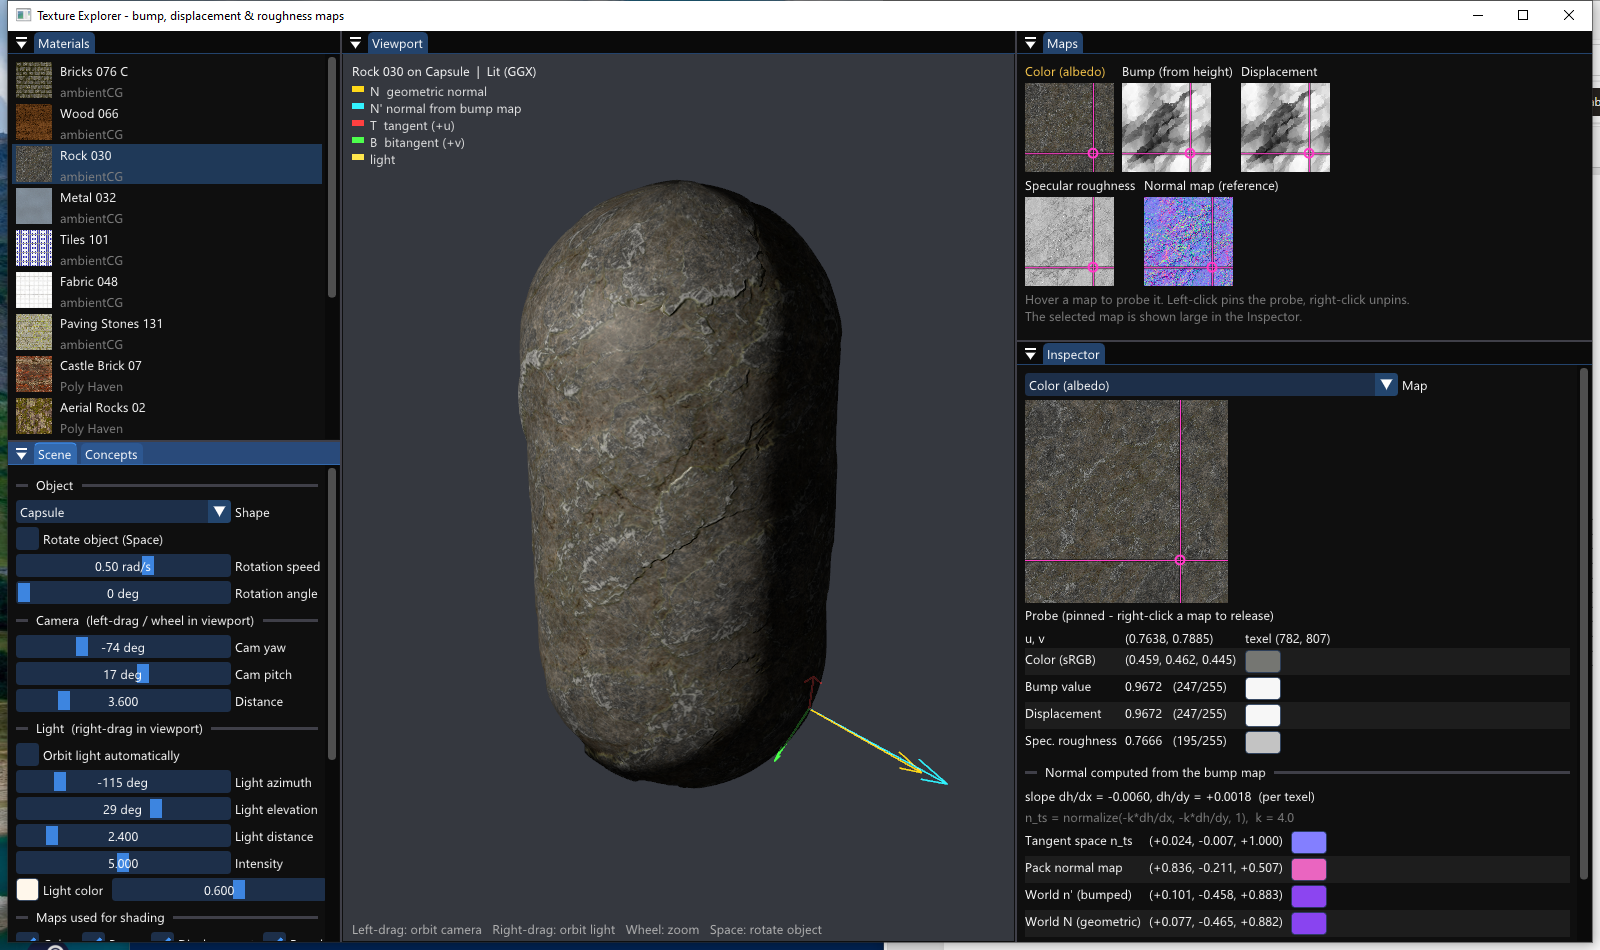
\includegraphics[width=\linewidth]{figures/capsule-roughness.png}
  \caption{The rock material on the capsule, with a pinned probe. Compare the
  ``Tangent space $n_{\mathrm{ts}}$'' row, computed from the bump map, with the ``Pack normal
  map'' row, decoded from the material's own normal map: the material's map was baked from
  much finer geometry, so here it leans far more strongly.}
  \label{fig:capsule}
\end{figure}

The Inspector lists, for the probed texel:
\begin{description}[font=\normalfont\itshape]
\item[u, v] the normalized coordinates and the integer texel;
\item[Color (sRGB)] the stored colour, with a swatch;
\item[Bump value, Displacement, Spec.\ roughness] as fractions and as stored bytes ($/255$);
\item[slope] $h_x$ and $h_y$ in height units per texel;
\item[Tangent space $n_{\mathrm{ts}}$] equation~\eqref{eq:nts}, with its colour encoding
$\frac12\vect n+\frac12$;
\item[Pack normal map] the material's own normal map at the same texel, decoded by
$2\,\mathit{rgb}-1$, for comparison (Section~\ref{sec:normalmaps});
\item[World $\vect n'$, World $\Nv$, World $\Tv$, World $\Bv$, World position] the bumped and the
geometric normals, the frame, and the displaced point, in world coordinates.
\end{description}
The same quantities appear in the 3D view as arrows (Figure~\ref{fig:pyramid}). The bumped normal
$\vect n'$ deviates from $\Nv$ by an angle that grows with the bump strength, and the frame
$\Tv,\Bv$ shows how the texture is laid on the surface at that point.

\chapter{The shaders}
\label{ch:shaders}

The GPU work is done by two short HLSL programs in \file{shaders/pbr.hlsl}. The program compiles
them at start-up and whenever the user presses F5, so students can edit the file while the
program runs. If a modified shader does not compile, the program keeps the previous version and
shows the compiler's messages in the Scene panel.

\section{The constant buffer}
All per-frame parameters travel in one constant buffer. HLSL packs constant buffers in rows of
16 bytes and does not let a vector straddle two rows, so the declaration is arranged in groups of
four scalars:

\excerpt{cbuffer}

The C++ structure that fills it must have exactly the same layout; a \code{static\_assert}
checks the most common mistake, a size that is not a multiple of 16:

\excerpt{frameconstants}

DirectXMath stores matrices by rows and multiplies row vectors on the left, $\vect p'=\vect pM$.
Declaring the HLSL matrices \code{row\_major} and writing \code{mul(p, M)} follows the same
convention, so no transposition is needed.

\section{Vertex shader: displacement}
\label{sec:vs}
The vertex shader is equation~\eqref{eq:displace}. It samples the displacement map at the mipmap
level \code{dispLod} chosen on the CPU (Chapter~\ref{ch:sampling}), moves the vertex along its
normal, and transforms position, normal and tangent to the world. It does \emph{not} recompute
the normal (Section~\ref{sec:displacement}).

\excerpt{vsmain}

\section{The bump normal on the GPU}
This is equation~\eqref{eq:nts} again, written to match the C++ version line by line:

\excerpt{bumpnormalts}

\section{Pixel shader: bump mapping and lighting}
The pixel shader proceeds in the order of the theory chapters:
\begin{enumerate}
\item Rebuild an orthonormal frame from the interpolated normal and tangent (Gram--Schmidt), and
the bitangent from the stored sign (Chapter~\ref{ch:tangent}).
\item Compute $\nts$ from the bump map and transform it with the TBN matrix.
\item Read the albedo (decoded from sRGB by the view) and the roughness, or the neutral values
chosen in the interface when a map is switched off.
\item Either output a debug view or evaluate the GGX/Cook--Torrance model of
Chapter~\ref{ch:lighting}, with the horizon factor.
\item Draw a magenta ring around the probed texel, in texture space.
\end{enumerate}

\excerpt{psmain}

Two details deserve a comment. The debug views write values such as $\frac12\vect n+\frac12$
that must reach the screen unchanged, but the render target encodes everything as sRGB; the
shader therefore applies the approximate inverse, $c^{2.2}$, beforehand. And the roughness is
clamped to at least $0.04$, because a perfectly smooth GGX surface has an infinitely thin
highlight that a point light cannot show.

\chapter{The renderer and the user interface}
\label{ch:renderer}

\section{Shaders that can be reloaded}
\code{ReloadShaders} compiles the four entry points from their files with
\code{D3DCompileFromFile}, collecting the compiler's messages in a log. It creates the new
shader objects and input layouts first, and replaces the old ones only if everything succeeded.
A typing mistake in a shader therefore leaves the program running with the previous version.
The input layouts use \code{offsetof} on the C++ vertex structures, so the structures are the
only description of the vertex format.

\excerpt{reloadshaders}

\section{The off-screen target}
The 3D view is rendered into a texture the size of the Viewport panel, which Dear ImGui then
shows like any other image. The target uses four samples per pixel (multisample antialiasing),
which smooths the silhouette of the solid and the thin lines of the probe. It is written through
an sRGB view, so the GPU encodes the linear colours of the lighting, and \emph{resolved} into a
single-sample texture that the interface reads through a plain view. This is the same
typeless-texture technique used for the colour maps (Section~\ref{sec:typeless}).

\excerpt{scenetarget}

\section{Drawing the scene}
\code{RenderScene} clears the target, uploads the constant buffer (with \code{WRITE\_DISCARD}, so
the CPU never waits for the GPU to finish the previous frame), and draws the surface with one
indexed draw call. The four maps are bound to both shader stages: the vertex shader needs the
displacement map. A missing map is replaced by a neutral grey texture.

The lines of the probe and of the light marker are drawn twice from the same buffer: first at
30\,\% opacity without the depth test, so that parts hidden behind the solid remain faintly
visible, then normally with the depth test. Finally the textures are unbound, because Direct3D
refuses to bind a resource for reading and writing at once, and the multisampled image is
resolved. The resolve uses the sRGB format, so the samples are averaged in linear light.

\excerpt{renderscene}

\section{The frame of the application}
\code{App::Frame} is the function of Figure~\ref{fig:frame}. The order matters in one respect:
the probe is decided while the map panels are built, before the viewport, which needs the
probe's result to draw the arrows.

\excerpt{frame}

\section{Images that answer the mouse}
Every image of a map in the interface (the tiles of the Maps panel and the large image of the
Inspector) is drawn by \code{App::MapImage}, which also converts the mouse position into texture
coordinates:
\[
  (u,v) = \Bigl(\frac{p_x-m_x}{W},\ \frac{p_y-m_y}{H}\Bigr)\ \text{clamped to }[0,1]^2,
\]
where $\vect m$ is the image's top-left corner on the screen and $(W,H)$ its size. Hovering moves
the probe, a left click pins it, a right click releases it. The probe's crosshair is drawn on
every map image, so the eye can compare the maps at the same texel.

\excerpt{mapimageui}

\section{Filling the constant buffer}
The Viewport panel computes the camera matrices (right-handed, looking at the origin) and copies
the application's state into the constant buffer. A map is used only if it is switched on
\emph{and} present, and the mipmap level for the displacement is chosen to match the mesh
resolution:

\excerpt{fillconstants}

\section{The main loop}
\file{main.cpp} creates the window, initializes Dear ImGui (with docking, and with its layout file
next to the executable), and runs the classic loop: process the window messages, measure the
elapsed time, build the interface (which renders the scene off-screen), draw the interface into
the window, and present it synchronized with the display.

\excerpt{mainloop}

\chapter{Experiments and exercises}
\label{ch:exercises}

\section{Experiments with the program}
These experiments need no programming. Each one connects something visible in the program to a
section of Part~I.

\begin{enumerate}[label=\textbf{E\arabic*.}]
\item \emph{Texture space} (Chapter~\ref{ch:texspace}). Select the ``UV coordinates'' view. On each
solid, locate $u=0$, $u=1$ and the seam; on the sphere, observe the pinching at the poles; on the
cylinder, explain why the caps show the same colours as parts of the side.
\item \emph{Normalized coordinates.} Hover over the corners of the large image in the Inspector and
check that $(u,v)$ goes from $(0,0)$ at the top left to $(1,1)$ at the bottom right, and that the
texel index is $\lfloor uW\rfloor$.
\item \emph{Bump versus displacement} (Chapter~\ref{ch:height}). With the sphere and a rough
material, untick ``Bump'' and look at the silhouette and the lighting. Then tick ``Bump'' and
untick ``Displacement''. Then increase ``Displacement scale'' to $0.3$ with bump off: why does the
surface look strangely smooth despite its jagged outline?
\item \emph{Cracks.} With displacement on, look at the edges of the pyramid and the rims of the
cylinder from close up. Explain the cracks with equation~\eqref{eq:displace}.
\item \emph{Bump strength} (Section~\ref{sec:bumpformula}). Pin the probe on a groove and read
$\nts$ while varying the bump strength from $0$ to $30$. Plot the angle between $\nts$ and
$(0,0,1)$ as a function of $k$ and compare with $\arctan\bigl(k\sqrt{h_x^2+h_y^2}\bigr)$.
\item \emph{Tangent space versus world space} (Chapter~\ref{ch:tangent}). Pin the probe and start
the rotation. Which numbers change and which do not? Then change the shape: which numbers change
now?
\item \emph{Normal maps} (Section~\ref{sec:normalmaps}). For several texels, compare the signs of
the $x$ and $y$ components of the computed $\nts$ and of the pack normal map. Do they agree? What
would happen with an OpenGL normal map?
\item \emph{Roughness} (Chapter~\ref{ch:lighting}). Untick ``Roughness'' and sweep the constant
roughness from $0.04$ to $1$ while the light orbits automatically. Relate the size of the
highlight to Figure~\ref{fig:ggx}.
\item \emph{Colour spaces} (Section~\ref{sec:srgb}). Compare the Inspector's ``Color (sRGB)'' value
of a mid-grey texel with the value that the lighting actually uses after decoding. How large is
the difference?
\end{enumerate}

\section{Programming exercises}
In increasing order of difficulty. After editing a shader, press F5; after editing C++,
rebuild.

\begin{enumerate}[label=\textbf{P\arabic*.}]
\item In \code{SpherePatches}, remove the minus signs of the $z$ components. Describe what
happens to the texture and to the Inspector's $\Tv$ and $\Bv$, and relate it to
equation~\eqref{eq:orientation} and to the sign $w$.
\item Replace the central differences by forward differences, both in \code{BumpNormalTS} and in
\code{BumpNormalTangent}. Compare the probe's normal before and after on a sharp edge.
\item Add a view mode that shows the angle between the bumped normal and the geometric normal as a
heat map.
\item Add a view mode that shows the difference between the normal computed from the bump map and
the material's normal map. (You will need to bind the normal map to a fifth texture slot.)
\item Make the bump strength physically correct by dividing by the local stretch of the
parametrization, $\lVert\vect P_u\rVert$ and $\lVert\vect P_v\rVert$
(Section~\ref{sec:bumpformula}). On which solid is the change most visible?
\item Recompute the normal in the vertex shader from the displacement map, so that displacement
alone produces correct shading.
\item Close the cracks of the pyramid by displacing the vertices of the edges along the average of
the normals of the two faces that meet there.
\item Replace vertex displacement by hardware tessellation (hull and domain shaders) with a
tessellation factor that depends on the distance to the camera.
\end{enumerate}

\part{The macOS port}
\chapter{The macOS port}
\label{ch:macport}

The folder \file{mac} of the repository contains a second implementation of Texture Explorer,
for macOS and Apple's graphics interface, Metal. It is the same program: the same panels and
controls, the same defaults, the same materials (the folder \file{assets} is shared) and, above
all, the same formulas. Figure~\ref{fig:macpyramid} shows it in the situation of
Figure~\ref{fig:pyramid}.

\begin{figure}[ht]
  \centering
  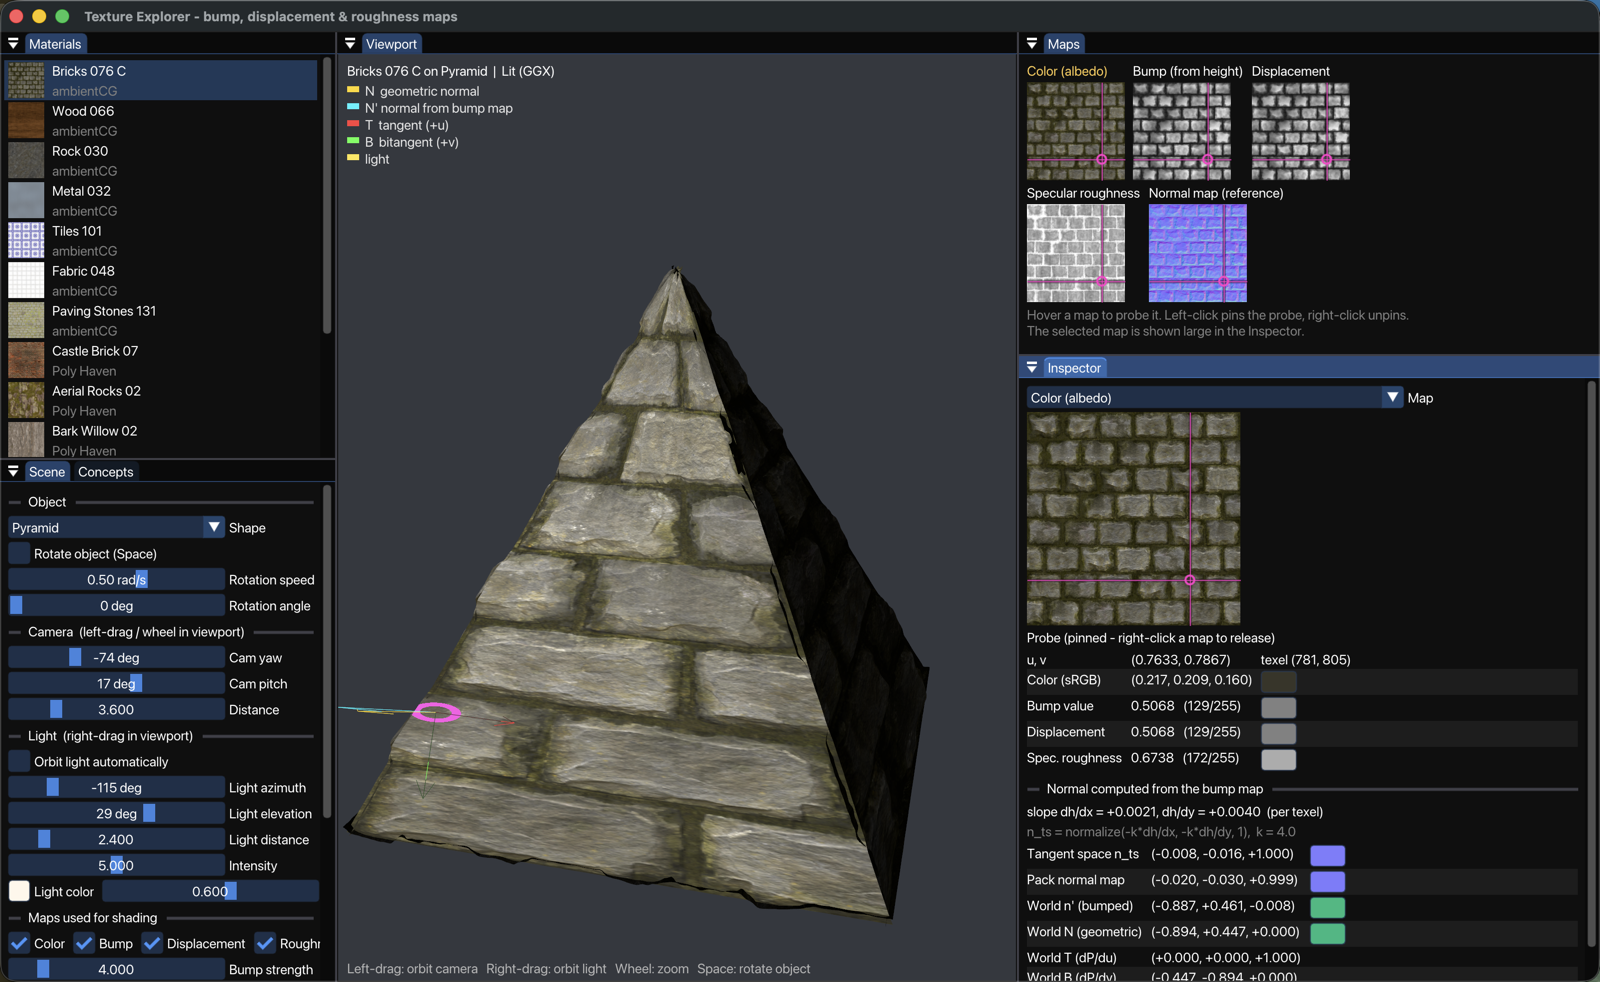
\includegraphics[width=\linewidth]{figures/pyramid-probe-mac.png}
  \caption{The macOS version in the situation of Figure~\ref{fig:pyramid}: same material,
  shape, camera and light, with the probe pinned near the same texel. The geometric normal
  $\Nv=(-0.894, 0.447, 0.000)$ is the same in both inspectors.}
  \label{fig:macpyramid}
\end{figure}

The port was written so that it can be read next to the original: every file of \file{src}
has a counterpart with the same name in \file{mac/src}, with the same classes and functions in
the same order. Only four layers of the program depend on the platform, and each is replaced
by its macOS counterpart (Table~\ref{tab:layers}). This chapter goes through them; the next
one explains how to compare the two implementations.

\begin{table}[ht]
\centering\small
\begin{tabularx}{\linewidth}{@{}lllX@{}}
\toprule
\textbf{Layer} & \textbf{Windows} & \textbf{macOS} & \textbf{Where}\\
\midrule
vectors and matrices & DirectXMath & \code{simd} & \file{mac/src/VecMath.h}, everywhere\\
GPU interface & Direct3D~11 & Metal (metal-cpp) & \file{Renderer.*}, \file{Material.cpp}\\
shading language & HLSL & Metal Shading Language & \file{mac/shaders/*.metal}\\
window and events & Win32 & AppKit, MetalKit & \file{main.mm}\\
\bottomrule
\end{tabularx}
\caption{The four platform layers of Texture Explorer. Dear ImGui, \code{stb\_image} and
\code{nlohmann/json} are used unchanged; ImGui has back ends for both systems.}
\label{tab:layers}
\end{table}

Metal is an Objective-C interface, but Apple publishes \emph{metal-cpp}, a header-only C++
wrapper in which every Metal object is a C++ class: \code{MTL::Device}, \code{MTL::Texture},
\code{MTL::RenderCommandEncoder}, and so on. With it, the whole port except \file{main.mm} is
plain C++20, and the Direct3D and Metal versions of a function can be compared line by line.

\section{Building and running}
The port needs macOS~13 or later, Xcode or its command-line tools, and CMake. The materials are
already in the repository. From its root:
\begin{lstlisting}[language={},numbers=none,frame=none,basicstyle=\ttfamily\small]
cmake -S mac -B mac/build -DCMAKE_BUILD_TYPE=Release
cmake --build mac/build
open mac/build/TextureExplorer.app
\end{lstlisting}
The controls are those of Chapter~\ref{ch:intro}; on a Mac the shaders are reloaded with F5
(fn-F5 on most keyboards) or Command-R. The program finds \file{assets} and
\file{mac/shaders} by walking up from the application bundle, so the shaders can be edited in
place while it runs.

\section{Vectors and matrices}
\label{sec:simd}
DirectXMath does not exist on macOS. Its replacement is Apple's \code{simd} library, whose types
\code{simd::float3}, \code{simd::float4x4}, \dots{} have the same names as the vector types of
the Metal Shading Language. Two differences matter.

\paragraph{Storage.} DirectXMath distinguishes a computing type, \code{XMVECTOR} (a SIMD
register), from storage types such as \code{XMFLOAT3} (three packed floats), and converts with
\code{XMLoadFloat3} and \code{XMStoreFloat3}. A \code{simd::float3} is both, but it occupies 16
bytes, so a vertex built from it would not have the packed 48-byte layout of the Direct3D
version. The port therefore computes with \code{simd::float3} and stores GPU data in two small
structures, \code{Float3} and \code{Float4}, which convert to and from \code{simd} implicitly.
The code becomes shorter: compare the sides of the pyramid in the two versions, where
\code{XMLoadFloat3}, \code{XMVectorLerp} and \code{XMStoreFloat3} simply disappear.

\paragraph{Row and column vectors.} DirectXMath multiplies a \emph{row} vector by a matrix,
$\vect p'=\vect pM$; \code{simd}, like Metal and most mathematics texts, multiplies a matrix by
a \emph{column} vector, $\vect p'=M\vect p$. Each matrix of one convention is the transpose of
the corresponding matrix of the other, and products are written in the opposite order:
\[
  \vect p_{\mathrm{clip}} = \vect p\,(W\,V\,P) \quad\text{(Windows)},\qquad
  \vect p_{\mathrm{clip}} = (P\,V\,W)\,\vect p \quad\text{(macOS)}.
\]
\file{mac/src/VecMath.h} defines the few constructors the program needs, each the transpose of
its DirectXMath namesake. For example, the view matrix has the camera's axes as its rows:

\excerpt{mlookat}

The projection matrix carries over unchanged because Metal shares two conventions with Direct3D:
clip-space depth runs from $0$ at the near plane to $1$ at the far plane (OpenGL uses $-1$ to
$1$), and the origin of a texture is its top-left corner, with $v$ growing downwards
(Section~\ref{sec:uvconv}). Everything that Part~I says about texture space therefore holds on
both systems, and the patch functions of Chapter~\ref{ch:geometry} are the same; only their
vector types change.

\excerpt{mperspective}

\section{From HLSL to the Metal Shading Language}
\label{sec:msl}
The Metal Shading Language (MSL) is a dialect of C++14 with vector types named like HLSL's,
so the translation of \file{shaders/pbr.hlsl} into \file{mac/shaders/pbr.metal} is close to
mechanical. Table~\ref{tab:hlslmsl} lists every kind of change it needed. The mathematics---the
displacement, the central differences, the TBN matrix, the GGX/Cook--Torrance BRDF---is
identical, statement by statement.

\begin{table}[ht]
\centering\small
\begin{tabularx}{\linewidth}{@{}>{\raggedright\arraybackslash}X>{\raggedright\arraybackslash}X@{}}
\toprule
\textbf{HLSL} (\file{shaders/pbr.hlsl}) & \textbf{MSL} (\file{mac/shaders/pbr.metal})\\
\midrule
\code{cbuffer Frame : register(b0) \{...\}} & \code{struct Frame \{...\}}, passed as \code{constant Frame\& f [[buffer(1)]]}\\
\code{Texture2D colorMap : register(t0);} (global) & \code{texture2d<float> colorMap [[texture(0)]]} (function parameter)\\
\code{SamplerState linearWrap : register(s0);} & \code{sampler linearWrap [[sampler(0)]]}\\
semantics \code{POSITION}, \code{NORMAL}, \dots & \code{[[attribute(0)]]}, \code{[[attribute(1)]]}, \dots{} with \code{[[stage\_in]]}\\
\code{SV\_Position}, \code{SV\_Target} & \code{[[position]]}; the return value of a \code{fragment} function\\
entry point chosen by the compiler call & keywords \code{vertex} and \code{fragment}\\
\code{mul(v, M)} with \code{row\_major} & \code{M * v}\\
\code{lerp}, \code{frac} & \code{mix}, \code{fract}\\
\code{t.SampleLevel(s, uv, l)} & \code{t.sample(s, uv, level(l))}\\
\code{t.GetDimensions(w, h)} & \code{t.get\_width()}, \code{t.get\_height()}\\
\code{r.xxx} (swizzle of a scalar) & \code{float3(r)}\\
\code{float3} in a constant buffer (12 bytes) & \code{packed\_float3} (a \code{float3} takes 16 bytes)\\
\bottomrule
\end{tabularx}
\caption{The changes made in translating the shaders from HLSL to MSL.}
\label{tab:hlslmsl}
\end{table}

\paragraph{Resources are parameters.} The most visible change is that textures, samplers and
constants are not global variables bound to registers but parameters of the shader functions,
with the binding number as an attribute. A helper function such as \code{BumpNormalTS} cannot see
the resources of its caller, so they are passed to it explicitly:

\excerpt{mbumpnormalts}

\paragraph{The layout of the constants.} An HLSL constant buffer packs a \code{float3} into 12
bytes and lets the next \code{float} complete the 16-byte row. In MSL, as in C++ with
\code{simd}, a \code{float3} is aligned to 16 bytes; MSL's \code{packed\_float3} restores the
HLSL behaviour. With it, the structure has the rows of the \code{cbuffer} of
Chapter~\ref{ch:shaders}, 240 bytes in both versions, and the C++ structure uses \code{Float3} in
the same places. Its \code{static\_assert} now checks the size and one offset exactly:

\excerpt{mframe}

\excerpt{mframeconstants}

The vertex shader shows the remaining differences: semantics replaced by attributes, the
constants reached through \code{f}, and products in the column order.

\excerpt{mvsmain}

\section{Textures}
\label{sec:mactextures}
Direct3D separates a texture (memory) from its \emph{views} (interpretations of that memory);
Section~\ref{sec:typeless} used a typeless texture with a \code{UNORM} view for the interface and
a \code{UNORM\_SRGB} view for shading. Metal has only textures, but a texture created with the
usage flag \code{PixelFormatView} can produce another texture that is a view of the same memory
with a different pixel format. The colour map is therefore an \code{RGBA8Unorm} texture plus an
\code{RGBA8Unorm\_sRGB} view of it, which decodes sRGB when sampled, exactly as in Direct3D.
The CPU copy for the inspector is unchanged.

\excerpt{mloadimage}

Two other differences appear here. The pixels are written with \code{replaceRegion} into a
\emph{managed} texture, one that has a copy the CPU can write (on a Mac with Apple silicon the
CPU and the GPU share the memory, and the copy costs nothing). And the mipmaps are generated by
a command recorded into a \emph{command buffer}, which brings us to the main difference between
the two interfaces.

\section{The renderer}
\label{sec:macrenderer}
Table~\ref{tab:d3dmetal} is a dictionary of the concepts the renderer uses. The deepest
difference is in its second row. A Direct3D~11 \emph{immediate context} executes every call as
it is made, as far as the program can tell. Metal makes the recording of GPU work explicit: the
program takes a \emph{command buffer} from a \emph{command queue}, records passes into it through
\emph{encoders}, and \emph{commits} it; the GPU executes committed buffers in order. In Texture
Explorer each frame has one command buffer, which receives first the render pass of the scene
and then the render pass of the interface.

\begin{table}[ht]
\centering\small
\begin{tabularx}{\linewidth}{@{}>{\raggedright\arraybackslash}X>{\raggedright\arraybackslash}X@{}}
\toprule
\textbf{Direct3D 11} (\file{src/Renderer.cpp}) & \textbf{Metal} (\file{mac/src/Renderer.cpp})\\
\midrule
\code{ID3D11Device} & \code{MTL::Device}\\
immediate context (\code{ID3D11DeviceContext}) & command queue, command buffers, encoders\\
swap chain, \code{Present} & drawables of the \code{MTKView}, \code{presentDrawable}\\
texture + shader resource view & texture, possibly a view of another texture\\
render target and depth-stencil views & attachments of a render pass descriptor\\
\code{ClearRenderTargetView} & load action \code{Clear}\\
\code{ResolveSubresource} & store action \code{MultisampleResolve}\\
shaders + input layout + blend state & one render pipeline state\\
input layout (\code{D3D11\_INPUT\_ELEMENT\_DESC}) & vertex descriptor (attributes by number)\\
rasterizer state & \code{setCullMode}, \code{setViewport} on the encoder\\
depth-stencil state, sampler state & the same, created from descriptors\\
dynamic constant buffer, \code{Map(WRITE\_DISCARD)} & \code{setVertexBytes}, \code{setFragmentBytes}\\
dynamic vertex buffer & a new buffer per frame\\
\code{D3DCompileFromFile} & \code{newLibrary} from source text\\
\code{ComPtr} & \code{NS::SharedPtr}\\
\bottomrule
\end{tabularx}
\caption{Direct3D~11 and Metal concepts used by the renderer.}
\label{tab:d3dmetal}
\end{table}

\paragraph{Pipeline states.} Direct3D~11 lets the program combine shaders, input layout, blend
state and target formats freely at draw time. Metal, like Direct3D~12 and Vulkan, requires the
combination to be declared in advance and compiled once into an immutable \emph{render pipeline
state}, which therefore also names the formats of the targets: four samples per pixel, an sRGB
colour target and a 32-bit depth buffer. The lines get a second pipeline state, which is the
first one with blending enabled.

\excerpt{mpipeline}

\paragraph{The off-screen target} has the same three parts as in Direct3D: a multisampled
colour texture, a multisampled depth texture and a resolved single-sample texture, with a
non-sRGB view of the latter for the interface.

\excerpt{mscenetarget}

\paragraph{Drawing.} A render pass states what happens to each attachment at its start
(\emph{load action}) and end (\emph{store action}). Clearing is a load action, and the resolve of
the multisampled image is a store action, so there is no \code{ClearRenderTargetView} and no
\code{ResolveSubresource}. The depth buffer is not needed after the pass and is not stored at
all, which saves memory traffic, particularly on Apple GPUs, which keep the attachments of a
pass in on-chip memory. The constants are copied into the command buffer with
\code{setVertexBytes} rather than written into a buffer, because Metal does not rename memory
behind the program's back as \code{Map(WRITE\_DISCARD)} does; for the same reason the lines go
into a new small buffer each frame. Nothing needs to be unbound at the end: Metal tracks by
itself which passes write and which read each resource.

\excerpt{mrenderscene}

\section{The window and the frame}
\label{sec:macframe}
The Windows program owns its main loop: it processes the window's messages and then draws a
frame, over and over. A Mac program is organized the other way round. The application object
of AppKit owns the loop, and the program supplies a \emph{delegate} whose methods are called
when something happens. Drawing is driven the same way: a \code{MTKView} owns the drawable
images of the window (the counterpart of the swap chain) and calls its delegate once per refresh
of the display. That method, in \file{main.mm}, replaces the body of the Windows loop:

\excerpt{mframeloop}

Asking the view for its render pass descriptor may wait until the display releases a drawable;
this ties the frame rate to the display, as \code{Present(vsync)} does on Windows. The
\code{@autoreleasepool} releases at the end of the frame every object that Metal and AppKit
returned without handing it to the program (the command buffer, the encoders, the
descriptors). \file{main.mm} is the only file in Objective-C++; the casts written
\code{(\_\_bridge T)p} convert between metal-cpp pointers and Objective-C references, which
designate the same objects.

\paragraph{Points and pixels.} One change in the interface has nothing to do with Metal. On
macOS, Dear ImGui measures the screen in \emph{points}, and a Retina display has two pixels per
point in each direction. The scene is therefore rendered at the size of the Viewport panel in
pixels---\code{DisplayFramebufferScale} times its size in points---and shown at its size in
points, so that it is as sharp as the Windows image. On Windows the factor is~1.

\excerpt{mviewportsize}

\chapter{Comparing the two implementations}
\label{ch:comparing}

Two implementations of one program are an opportunity: whatever differs between them depends
on the platform, and whatever is common does not. This chapter describes three ways to compare
Direct3D and Metal versions of Texture Explorer, from the most informal to the most precise:
reading the code, running both programs, and measuring their results.

\section{Reading the code side by side}
Every source file has a counterpart with the same name, the same functions and the same order
(Table~\ref{tab:pairs}), so the two can be opened next to each other in any editor, or compared
with a difference tool from the root of the repository:
\begin{lstlisting}[language={},numbers=none,frame=none,basicstyle=\ttfamily\small]
git diff --no-index src/Inspector.cpp mac/src/Inspector.cpp
git diff --no-index --word-diff shaders/pbr.hlsl mac/shaders/pbr.metal
\end{lstlisting}
The amount of difference is itself instructive. The geometry and the inspector differ only in
vector types; the shaders only in the syntax of Table~\ref{tab:hlslmsl}; the user interface in a
handful of lines; the renderer and the main program almost everywhere.

\begin{table}[ht]
\centering\small
\begin{tabularx}{\linewidth}{@{}ll>{\raggedright\arraybackslash}X@{}}
\toprule
\textbf{Windows} & \textbf{macOS} & \textbf{What differs}\\
\midrule
--- & \file{mac/src/VecMath.h} & the parts of DirectXMath the program needs (Section~\ref{sec:simd})\\
\file{src/Mesh.*} & \file{mac/src/Mesh.*} & vector types only\\
\file{src/Material.*} & \file{mac/src/Material.*} & Metal textures and views; command buffer for mipmaps\\
\file{src/Inspector.*} & \file{mac/src/Inspector.*} & vector types only\\
\file{shaders/pbr.hlsl} & \file{mac/shaders/pbr.metal} & HLSL syntax $\to$ MSL syntax (Table~\ref{tab:hlslmsl})\\
\file{shaders/gizmo.hlsl} & \file{mac/shaders/gizmo.metal} & idem\\
\file{src/Renderer.*} & \file{mac/src/Renderer.*} & Direct3D~11 $\to$ Metal (Table~\ref{tab:d3dmetal})\\
\file{src/App.*} & \file{mac/src/App.*} & texture handles, paths, opening a URL, Retina scale, Command-R\\
\file{src/main.cpp} & \file{mac/src/main.mm} & Win32 loop $\to$ AppKit delegate and \code{MTKView}\\
\file{CMakeLists.txt} & \file{mac/CMakeLists.txt} & back ends of ImGui, metal-cpp, frameworks, bundle\\
\bottomrule
\end{tabularx}
\caption{The files of the two implementations.}
\label{tab:pairs}
\end{table}

The literate version of the program in \file{LiterateP} makes this comparison precise. It
contains both implementations, and every piece of code that is identical in both is written
once and \emph{used} by both: the woven document says so under the piece, and its index lists
all of them. Since the tool that checks the literate program regenerates both implementations
from it and compares them with the repository byte for byte, the list of shared pieces cannot
become outdated.

\section{Running both programs}
Both programs start with the same material, shape, camera, light and settings, and lay out their
panels the same way; Figures~\ref{fig:pyramid} and~\ref{fig:macpyramid} were taken that way. To
compare them:
\begin{enumerate}
\item Start both programs and choose the same material, shape and view mode.
\item Pin the probe on the same texel. Clicking in the large image of the Inspector is easiest;
the $(u,v)$ shown tells how close the two probes are.
\item Compare the readouts. The values of the maps and the tangent-space normal depend only on
$(u,v)$ and must agree to the digits shown; the world-space vectors depend also on the shape and
on the rotation, which can be set to the same angle with its slider.
\item Compare the images, in the lit view and in the debug views. The ``UV coordinates'',
``World normal'' and ``Tangent-space normal'' views turn the data of the shaders into colours,
so a screenshot of each can be compared pixel by pixel with an image tool.
\end{enumerate}
The images will be almost but not exactly identical, and the reasons are worth discussing:
\begin{itemize}
\item Neither Direct3D nor Metal requires bit-identical results from different GPUs. Texture
filtering, in particular anisotropic filtering, multisample coverage and the precision of
functions such as \code{pow} and \code{normalize} are specified only up to a tolerance.
\item The lines of the arrows are one \emph{pixel} wide, so they look half as thick on a Retina
display.
\item The fonts differ (Segoe~UI and San Francisco), and with them the sizes of the panels in
pixels.
\end{itemize}

\section{Measuring: the comparison program}
\label{sec:probe}
The CPU half of the program---the shapes, the sampling of the maps and the inspector---can be
compared exactly, and \file{mac/compare} contains a program that does it on a Mac. The obstacle
is that the two implementations never run on the same computer. However, the CPU half of the
Windows version needs only standard C++, DirectXMath and a few declarations from Direct3D.
DirectXMath is a header-only library that Microsoft publishes for other platforms too, and the
Direct3D declarations can be replaced by stand-ins that compile and do nothing. So the very files
\file{src/Mesh.cpp}, \file{src/Material.cpp} and \file{src/Inspector.cpp}, unmodified, can be
compiled on a Mac next to their macOS counterparts:
\begin{lstlisting}[language={},numbers=none,frame=none,basicstyle=\ttfamily\small]
cmake -S mac/compare -B mac/compare/build
cmake --build mac/compare/build --target compare
\end{lstlisting}

\paragraph{How it works.} The source file \file{probe.cpp} is compiled twice: once with the
Windows files (and the stand-ins of \file{mac/compare/shims} first in the include path), and once
with the files of the port. Both programs print the same report: the size of each mesh, every
997th vertex, and the full answer of the inspector---colour, bump, displacement, roughness,
slope, $\nts$, and the world-space position, $\Nv$, $\vect n'$, $\Tv$ and $\Bv$---for all ten
materials on all four shapes, at the corners of an $8\times8$ grid of texels (where wrapping
matters) and on a second grid between texel centres (where interpolation matters). The script
\file{compare.py} matches the two reports line by line and prints, for each quantity, the largest
difference. The stand-in for Direct3D is itself instructive: it lists exactly how much of
Direct3D the loading of a material touches.

\excerpt{shimdevice}

\paragraph{Results.} At the time of writing, the 7\,149 lines of the two reports compare as
follows:

\begin{center}\small
\begin{tabular}{@{}lr@{}}
\toprule
\textbf{Quantity} & \textbf{Largest difference}\\
\midrule
mesh sizes and index sums & identical\\
vertex positions, normals and tangents & $2\cdot10^{-7}$\\
vertex texture coordinates & $0$\\
colour, bump, displacement and roughness at the probe & $0$\\
slope of the height field & $0$\\
tangent-space normal $\nts$ & $2\cdot10^{-7}$\\
world-space $\Nv$, $\vect n'$, $\Tv$, $\Bv$ & $2\cdot10^{-7}$\\
world-space position of the probe & $1\cdot10^{-6}$\\
\bottomrule
\end{tabular}
\end{center}

The values read from the maps agree exactly, because both versions sample them with the same
statements (Section~\ref{sec:cpusampling}). The vectors differ in the last one or two bits of a
\code{float}, $2^{-23}\approx1.2\cdot10^{-7}$: DirectXMath and \code{simd} perform the same
operations, but not always in the same way---a normalization may divide by a square root in one
library and multiply by a reciprocal square root in the other. The script accepts differences up
to $10^{-5}$, a hundred times the rounding differences and far below anything visible in the
inspector, and fails otherwise. A real discrepancy is much larger: replacing the factor
$\frac12$ of the central differences by $0.6$ in one version makes the script fail with a
difference of $0.03$ in the slope, and it names the material, shape and texel where the largest
difference occurs.

\section{Exercises}
\begin{enumerate}[label=\textbf{C\arabic*.}]
\item Change the bump normal in one version only, for example to forward differences
(Section~\ref{sec:centraldiff}), and run the comparison. Which quantities does it flag? Why does
the slope change but not the values of the maps?
\item Compare \file{shaders/pbr.hlsl} and \file{mac/shaders/pbr.metal} with a word difference.
Classify every difference into the rows of Table~\ref{tab:hlslmsl}. Is there any difference in the
mathematics?
\item In \file{mac/shaders/pbr.metal}, replace one \code{packed\_float3} of \code{Frame} by
\code{float3}. Predict what happens on the screen, and explain why the \code{static\_assert} of
the C++ structure does not detect the mistake.
\item In the macOS viewport, write \code{view * proj} instead of \code{proj * view}. Describe the
image, and explain why the Windows version writes the product in the other order.
\item On a Retina display, render the scene at the size of the panel in points instead of pixels.
How does the image change, and why?
\item Capture the ``World normal'' view in both programs at the same window size and compute the
difference image. Where are the differences largest, and why there?
\item The comparison program covers only the CPU half. Design a comparison of the GPU half:
what would each program have to write to a file, and what tolerance would be reasonable?
\end{enumerate}

\appendix
\chapter{The materials}
\label{app:materials}

All ten materials are released under the Creative Commons CC0~1.0 licence (public domain
dedication), which allows any use without attribution; the program and this guide credit them
anyway. Each material is used at 1K resolution ($1024\times1024$).

\begin{table}[ht]
\centering\small
\begin{tabularx}{\linewidth}{@{}llX@{}}
\toprule
\textbf{Material} & \textbf{Source} & \textbf{Page}\\
\midrule
Bricks 076 C      & ambientCG  & \url{https://ambientcg.com/view?id=Bricks076C}\\
Wood 066          & ambientCG  & \url{https://ambientcg.com/view?id=Wood066}\\
Rock 030          & ambientCG  & \url{https://ambientcg.com/view?id=Rock030}\\
Metal 032         & ambientCG  & \url{https://ambientcg.com/view?id=Metal032}\\
Tiles 101         & ambientCG  & \url{https://ambientcg.com/view?id=Tiles101}\\
Fabric 048        & ambientCG  & \url{https://ambientcg.com/view?id=Fabric048}\\
Paving Stones 131 & ambientCG  & \url{https://ambientcg.com/view?id=PavingStones131}\\
Castle Brick 07   & Poly Haven (Rob Tuytel) & \url{https://polyhaven.com/a/castle_brick_07}\\
Aerial Rocks 02   & Poly Haven (Rob Tuytel) & \url{https://polyhaven.com/a/aerial_rocks_02}\\
Bark Willow 02    & Poly Haven (Charlotte Baglioni) & \url{https://polyhaven.com/a/bark_willow_02}\\
\bottomrule
\end{tabularx}
\caption{The materials of Texture Explorer and their origin.}
\end{table}

\chapter{Building this document}
\label{app:build}

The sources of this guide are in the \file{Docs} folder of the repository:
\begin{description}[font=\normalfont\ttfamily]
\item[guide.tex] the main file, with the preamble and the list of chapters;
\item[chapters/] one file per chapter;
\item[figures/] screenshots of the program (the diagrams are drawn with TikZ and pgfplots in
the chapters themselves);
\item[excerpts.txt] the list of code excerpts: for each, a source file and a regular expression
for its first line;
\item[build.ps1] the build script.
\end{description}
The build script first extracts each excerpt from the current sources into \file{build/excerpts},
following the braces of the function or structure that starts at the matching line. It then runs
\code{latexmk}, \code{pdflatex} or \code{tectonic}, whichever it finds, and writes
\file{TextureExplorer-Guide.pdf}:
\begin{lstlisting}[language={},numbers=none,basicstyle=\ttfamily\small]
powershell -ExecutionPolicy Bypass -File Docs\build.ps1
powershell -ExecutionPolicy Bypass -File Docs\build.ps1 -TeX C:\tools\tectonic.exe
\end{lstlisting}
On macOS or Linux the same script runs with PowerShell~7 (\code{brew install --cask powershell},
and \code{brew install tectonic} for a TeX engine):
\begin{lstlisting}[language={},numbers=none,basicstyle=\ttfamily\small]
pwsh Docs/build.ps1
\end{lstlisting}
Because the listings are extracted at build time, the guide always shows the code as it is. If a
function is renamed, the build stops with an error that names the excerpt to fix.

The repository also contains, in \file{LiterateP}, the complete program written as a literate
program in the style of Donald Knuth, from which every source file can be regenerated. That
document follows the code; this one follows the theory.

\begin{thebibliography}{99}
\addcontentsline{toc}{chapter}{References}

\bibitem{akenine2018}
T.~Akenine-M\"oller, E.~Haines, N.~Hoffman, A.~Pesce, M.~Iwanicki and S.~Hillaire.
\emph{Real-Time Rendering}, 4th edition. CRC Press, 2018.

\bibitem{blinn1978}
J.~F.~Blinn. Simulation of wrinkled surfaces.
\emph{Computer Graphics (Proceedings of SIGGRAPH~78)}, 12(3):286--292, 1978.

\bibitem{cook1984}
R.~L.~Cook. Shade trees.
\emph{Computer Graphics (Proceedings of SIGGRAPH~84)}, 18(3):223--231, 1984.

\bibitem{cook1982}
R.~L.~Cook and K.~E.~Torrance. A reflectance model for computer graphics.
\emph{ACM Transactions on Graphics}, 1(1):7--24, 1982.

\bibitem{heitz2014}
E.~Heitz. Understanding the masking-shadowing function in microfacet-based BRDFs.
\emph{Journal of Computer Graphics Techniques}, 3(2):48--107, 2014.

\bibitem{karis2013}
B.~Karis. Real shading in Unreal Engine~4.
\emph{SIGGRAPH 2013 Course: Physically Based Shading in Theory and Practice}, 2013.

\bibitem{mikkelsen2008}
M.~S.~Mikkelsen. \emph{Simulation of wrinkled surfaces revisited}.
Master's thesis, University of Copenhagen, 2008.

\bibitem{pharr2016}
M.~Pharr, W.~Jakob and G.~Humphreys.
\emph{Physically Based Rendering: From Theory to Implementation}, 3rd edition.
Morgan Kaufmann, 2016.

\bibitem{schlick1994}
C.~Schlick. An inexpensive BRDF model for physically-based rendering.
\emph{Computer Graphics Forum}, 13(3):233--246, 1994.

\bibitem{walter2007}
B.~Walter, S.~R.~Marschner, H.~Li and K.~E.~Torrance.
Microfacet models for refraction through rough surfaces.
In \emph{Proceedings of the Eurographics Symposium on Rendering}, 2007.

\bibitem{williams1983}
L.~Williams. Pyramidal parametrics.
\emph{Computer Graphics (Proceedings of SIGGRAPH~83)}, 17(3):1--11, 1983.

\end{thebibliography}

\end{document}
